\documentclass[]{book}
\usepackage{lmodern}
\usepackage{amssymb,amsmath}
\usepackage{ifxetex,ifluatex}
\usepackage{fixltx2e} % provides \textsubscript
\ifnum 0\ifxetex 1\fi\ifluatex 1\fi=0 % if pdftex
  \usepackage[T1]{fontenc}
  \usepackage[utf8]{inputenc}
\else % if luatex or xelatex
  \ifxetex
    \usepackage{mathspec}
  \else
    \usepackage{fontspec}
  \fi
  \defaultfontfeatures{Ligatures=TeX,Scale=MatchLowercase}
\fi
% use upquote if available, for straight quotes in verbatim environments
\IfFileExists{upquote.sty}{\usepackage{upquote}}{}
% use microtype if available
\IfFileExists{microtype.sty}{%
\usepackage{microtype}
\UseMicrotypeSet[protrusion]{basicmath} % disable protrusion for tt fonts
}{}
\usepackage[margin=1in]{geometry}
\usepackage{hyperref}
\PassOptionsToPackage{usenames,dvipsnames}{color} % color is loaded by hyperref
\hypersetup{unicode=true,
            pdftitle={A Knowledge Ecosystem - Deep Learning and Education},
            pdfauthor={Fanli Zheng (Christian) \& Haohan Wang},
            colorlinks=true,
            linkcolor=Maroon,
            citecolor=Blue,
            urlcolor=Blue,
            breaklinks=true}
\urlstyle{same}  % don't use monospace font for urls
\usepackage{natbib}
\bibliographystyle{apalike}
\usepackage{longtable,booktabs}
\usepackage{graphicx,grffile}
\makeatletter
\def\maxwidth{\ifdim\Gin@nat@width>\linewidth\linewidth\else\Gin@nat@width\fi}
\def\maxheight{\ifdim\Gin@nat@height>\textheight\textheight\else\Gin@nat@height\fi}
\makeatother
% Scale images if necessary, so that they will not overflow the page
% margins by default, and it is still possible to overwrite the defaults
% using explicit options in \includegraphics[width, height, ...]{}
\setkeys{Gin}{width=\maxwidth,height=\maxheight,keepaspectratio}
\IfFileExists{parskip.sty}{%
\usepackage{parskip}
}{% else
\setlength{\parindent}{0pt}
\setlength{\parskip}{6pt plus 2pt minus 1pt}
}
\setlength{\emergencystretch}{3em}  % prevent overfull lines
\providecommand{\tightlist}{%
  \setlength{\itemsep}{0pt}\setlength{\parskip}{0pt}}
\setcounter{secnumdepth}{5}
% Redefines (sub)paragraphs to behave more like sections
\ifx\paragraph\undefined\else
\let\oldparagraph\paragraph
\renewcommand{\paragraph}[1]{\oldparagraph{#1}\mbox{}}
\fi
\ifx\subparagraph\undefined\else
\let\oldsubparagraph\subparagraph
\renewcommand{\subparagraph}[1]{\oldsubparagraph{#1}\mbox{}}
\fi

%%% Use protect on footnotes to avoid problems with footnotes in titles
\let\rmarkdownfootnote\footnote%
\def\footnote{\protect\rmarkdownfootnote}

%%% Change title format to be more compact
\usepackage{titling}

% Create subtitle command for use in maketitle
\newcommand{\subtitle}[1]{
  \posttitle{
    \begin{center}\large#1\end{center}
    }
}

\setlength{\droptitle}{-2em}

  \title{A Knowledge Ecosystem - Deep Learning and Education}
    \pretitle{\vspace{\droptitle}\centering\huge}
  \posttitle{\par}
    \author{Fanli Zheng (Christian) \& Haohan Wang}
    \preauthor{\centering\large\emph}
  \postauthor{\par}
      \predate{\centering\large\emph}
  \postdate{\par}
    \date{{[}DRAFT{]} 2018-11-17}

\usepackage{booktabs}

\usepackage{amsthm}
\newtheorem{theorem}{Theorem}[chapter]
\newtheorem{lemma}{Lemma}[chapter]
\theoremstyle{definition}
\newtheorem{definition}{Definition}[chapter]
\newtheorem{corollary}{Corollary}[chapter]
\newtheorem{proposition}{Proposition}[chapter]
\theoremstyle{definition}
\newtheorem{example}{Example}[chapter]
\theoremstyle{definition}
\newtheorem{exercise}{Exercise}[chapter]
\theoremstyle{remark}
\newtheorem*{remark}{Remark}
\newtheorem*{solution}{Solution}
\begin{document}
\maketitle

{
\hypersetup{linkcolor=black}
\setcounter{tocdepth}{1}
\tableofcontents
}
\chapter*{Preface}\label{preface}
\addcontentsline{toc}{chapter}{Preface}

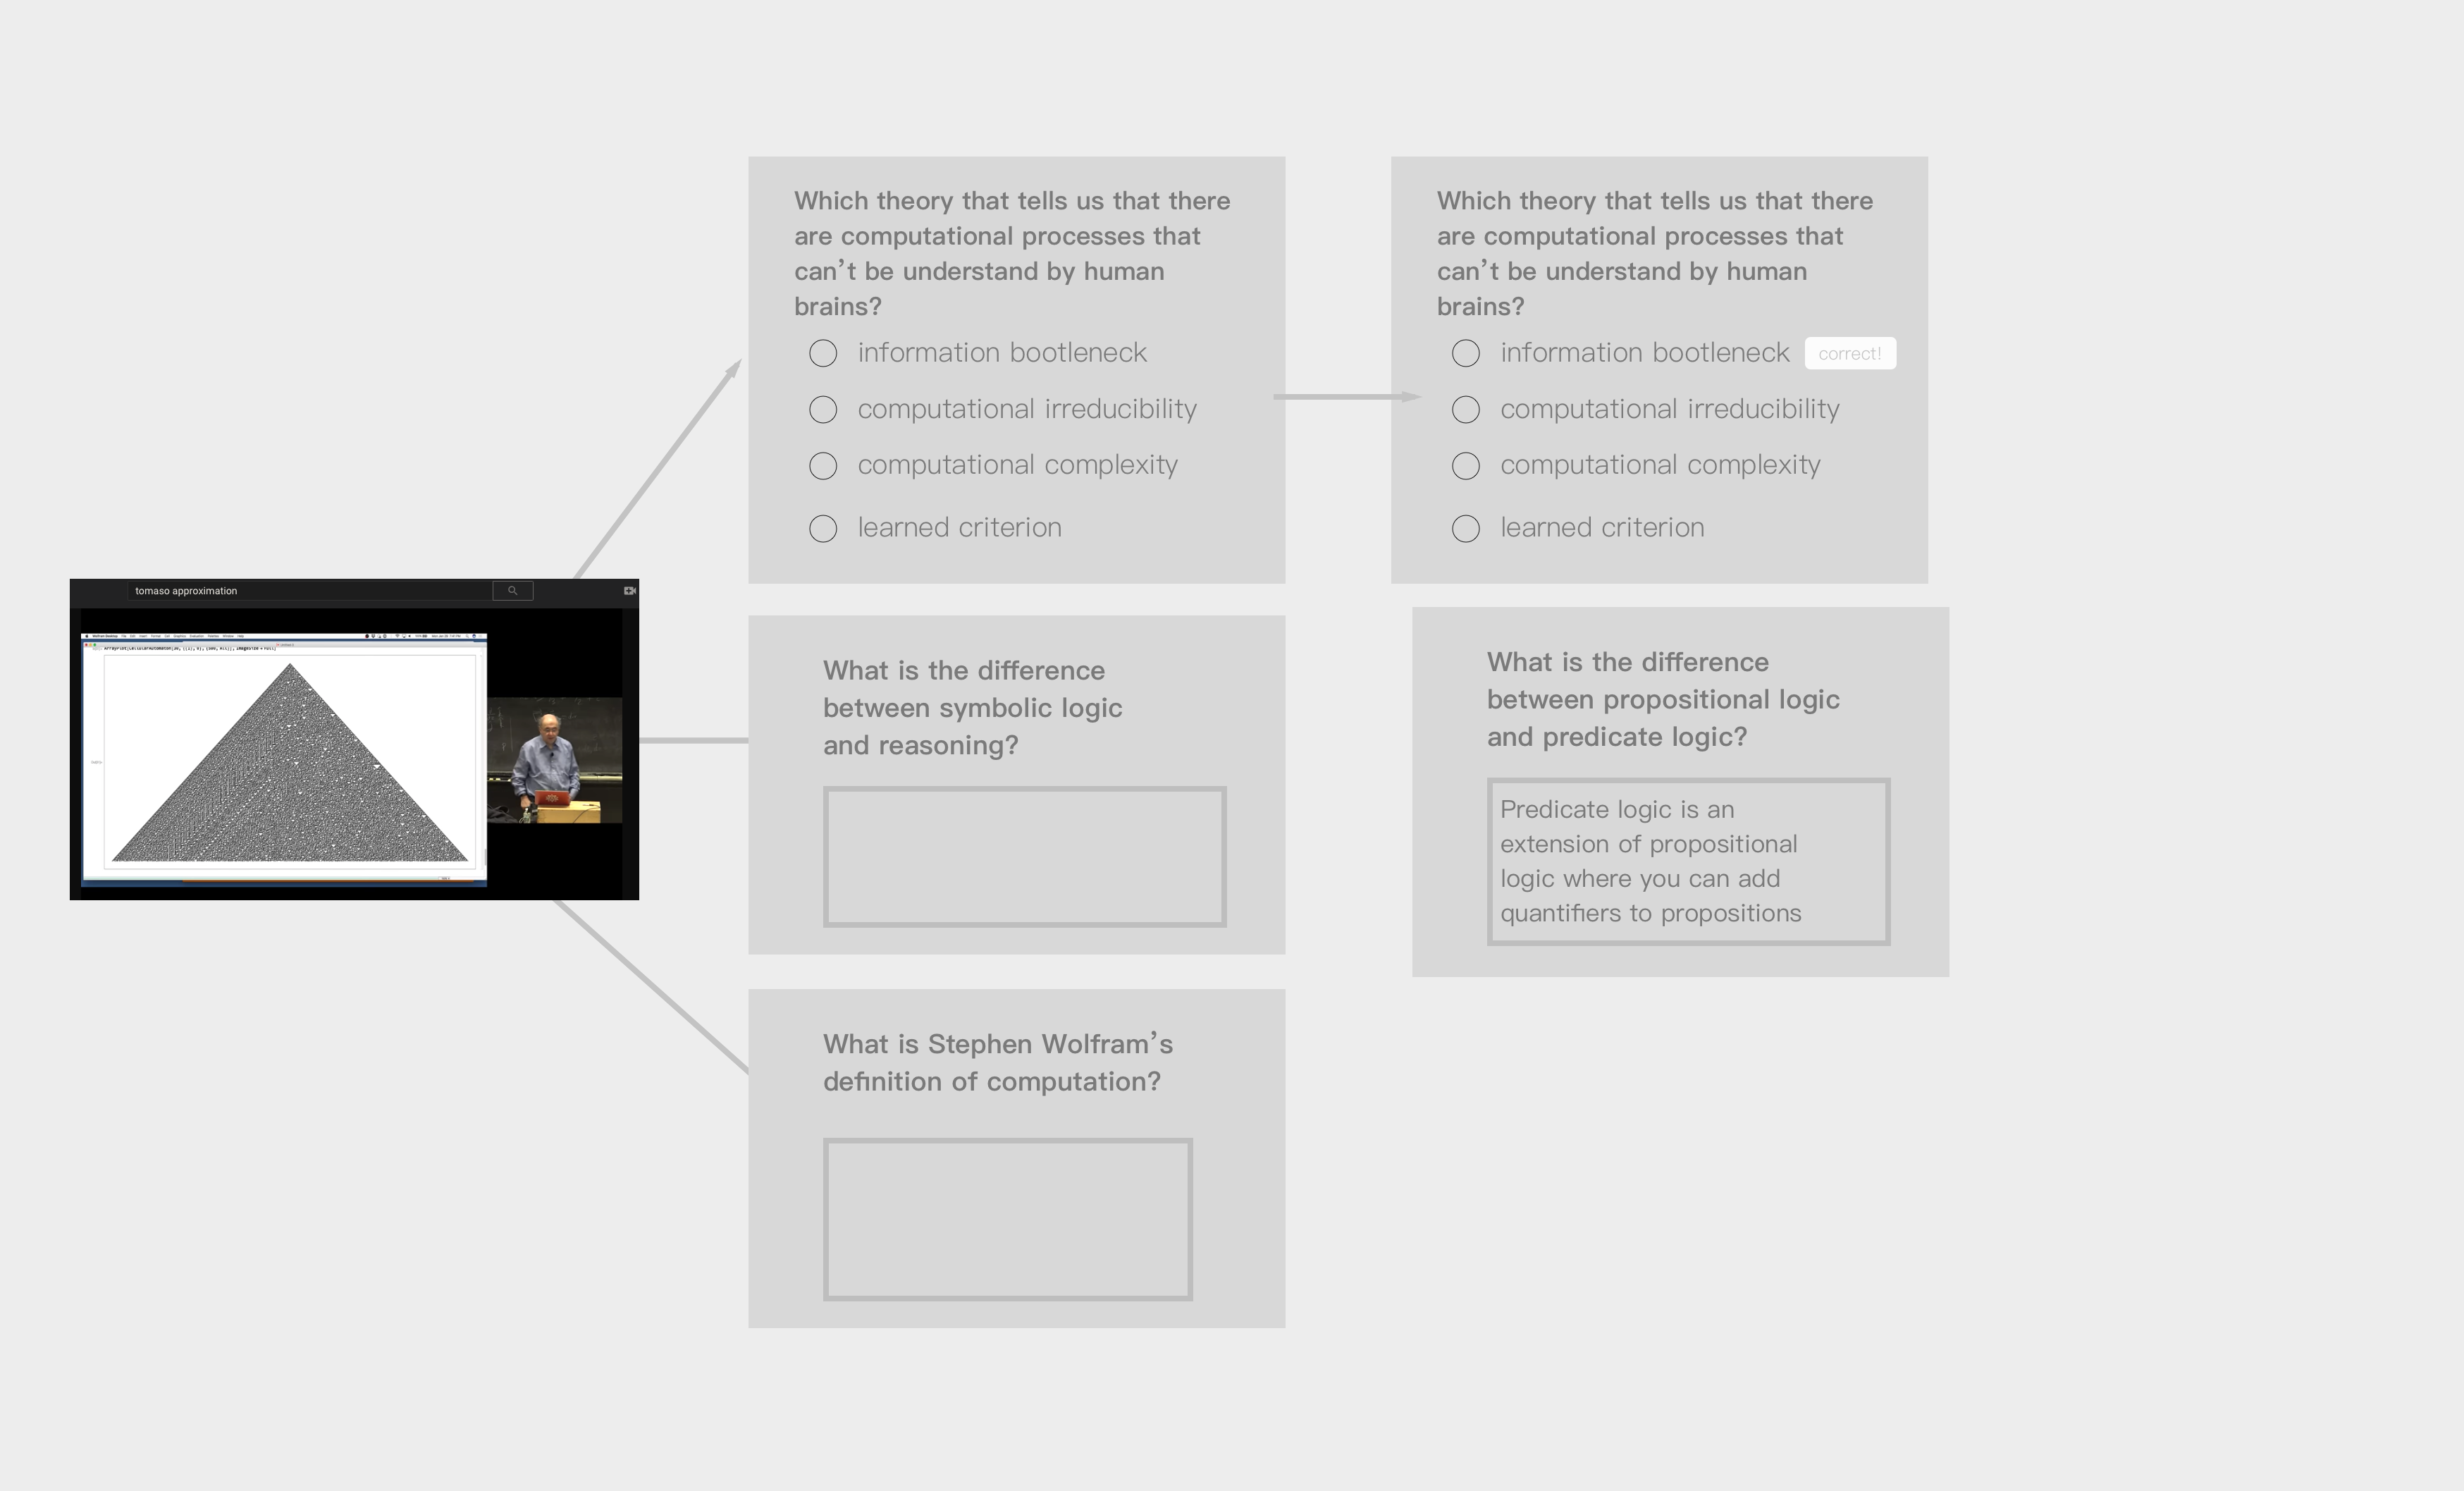
\includegraphics{img/MtoQA.png}
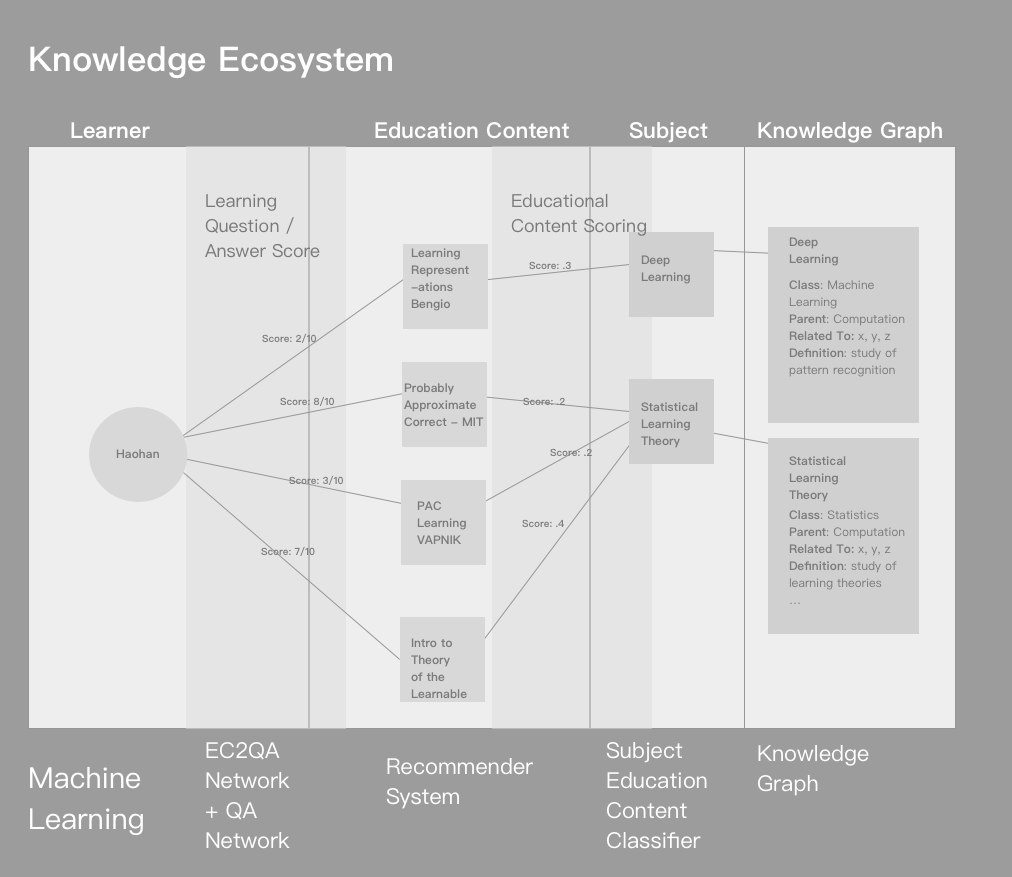
\includegraphics{img/knowledgeEcosystem.png}

\chapter{Introduction}\label{introduction}

\begin{figure}
\centering
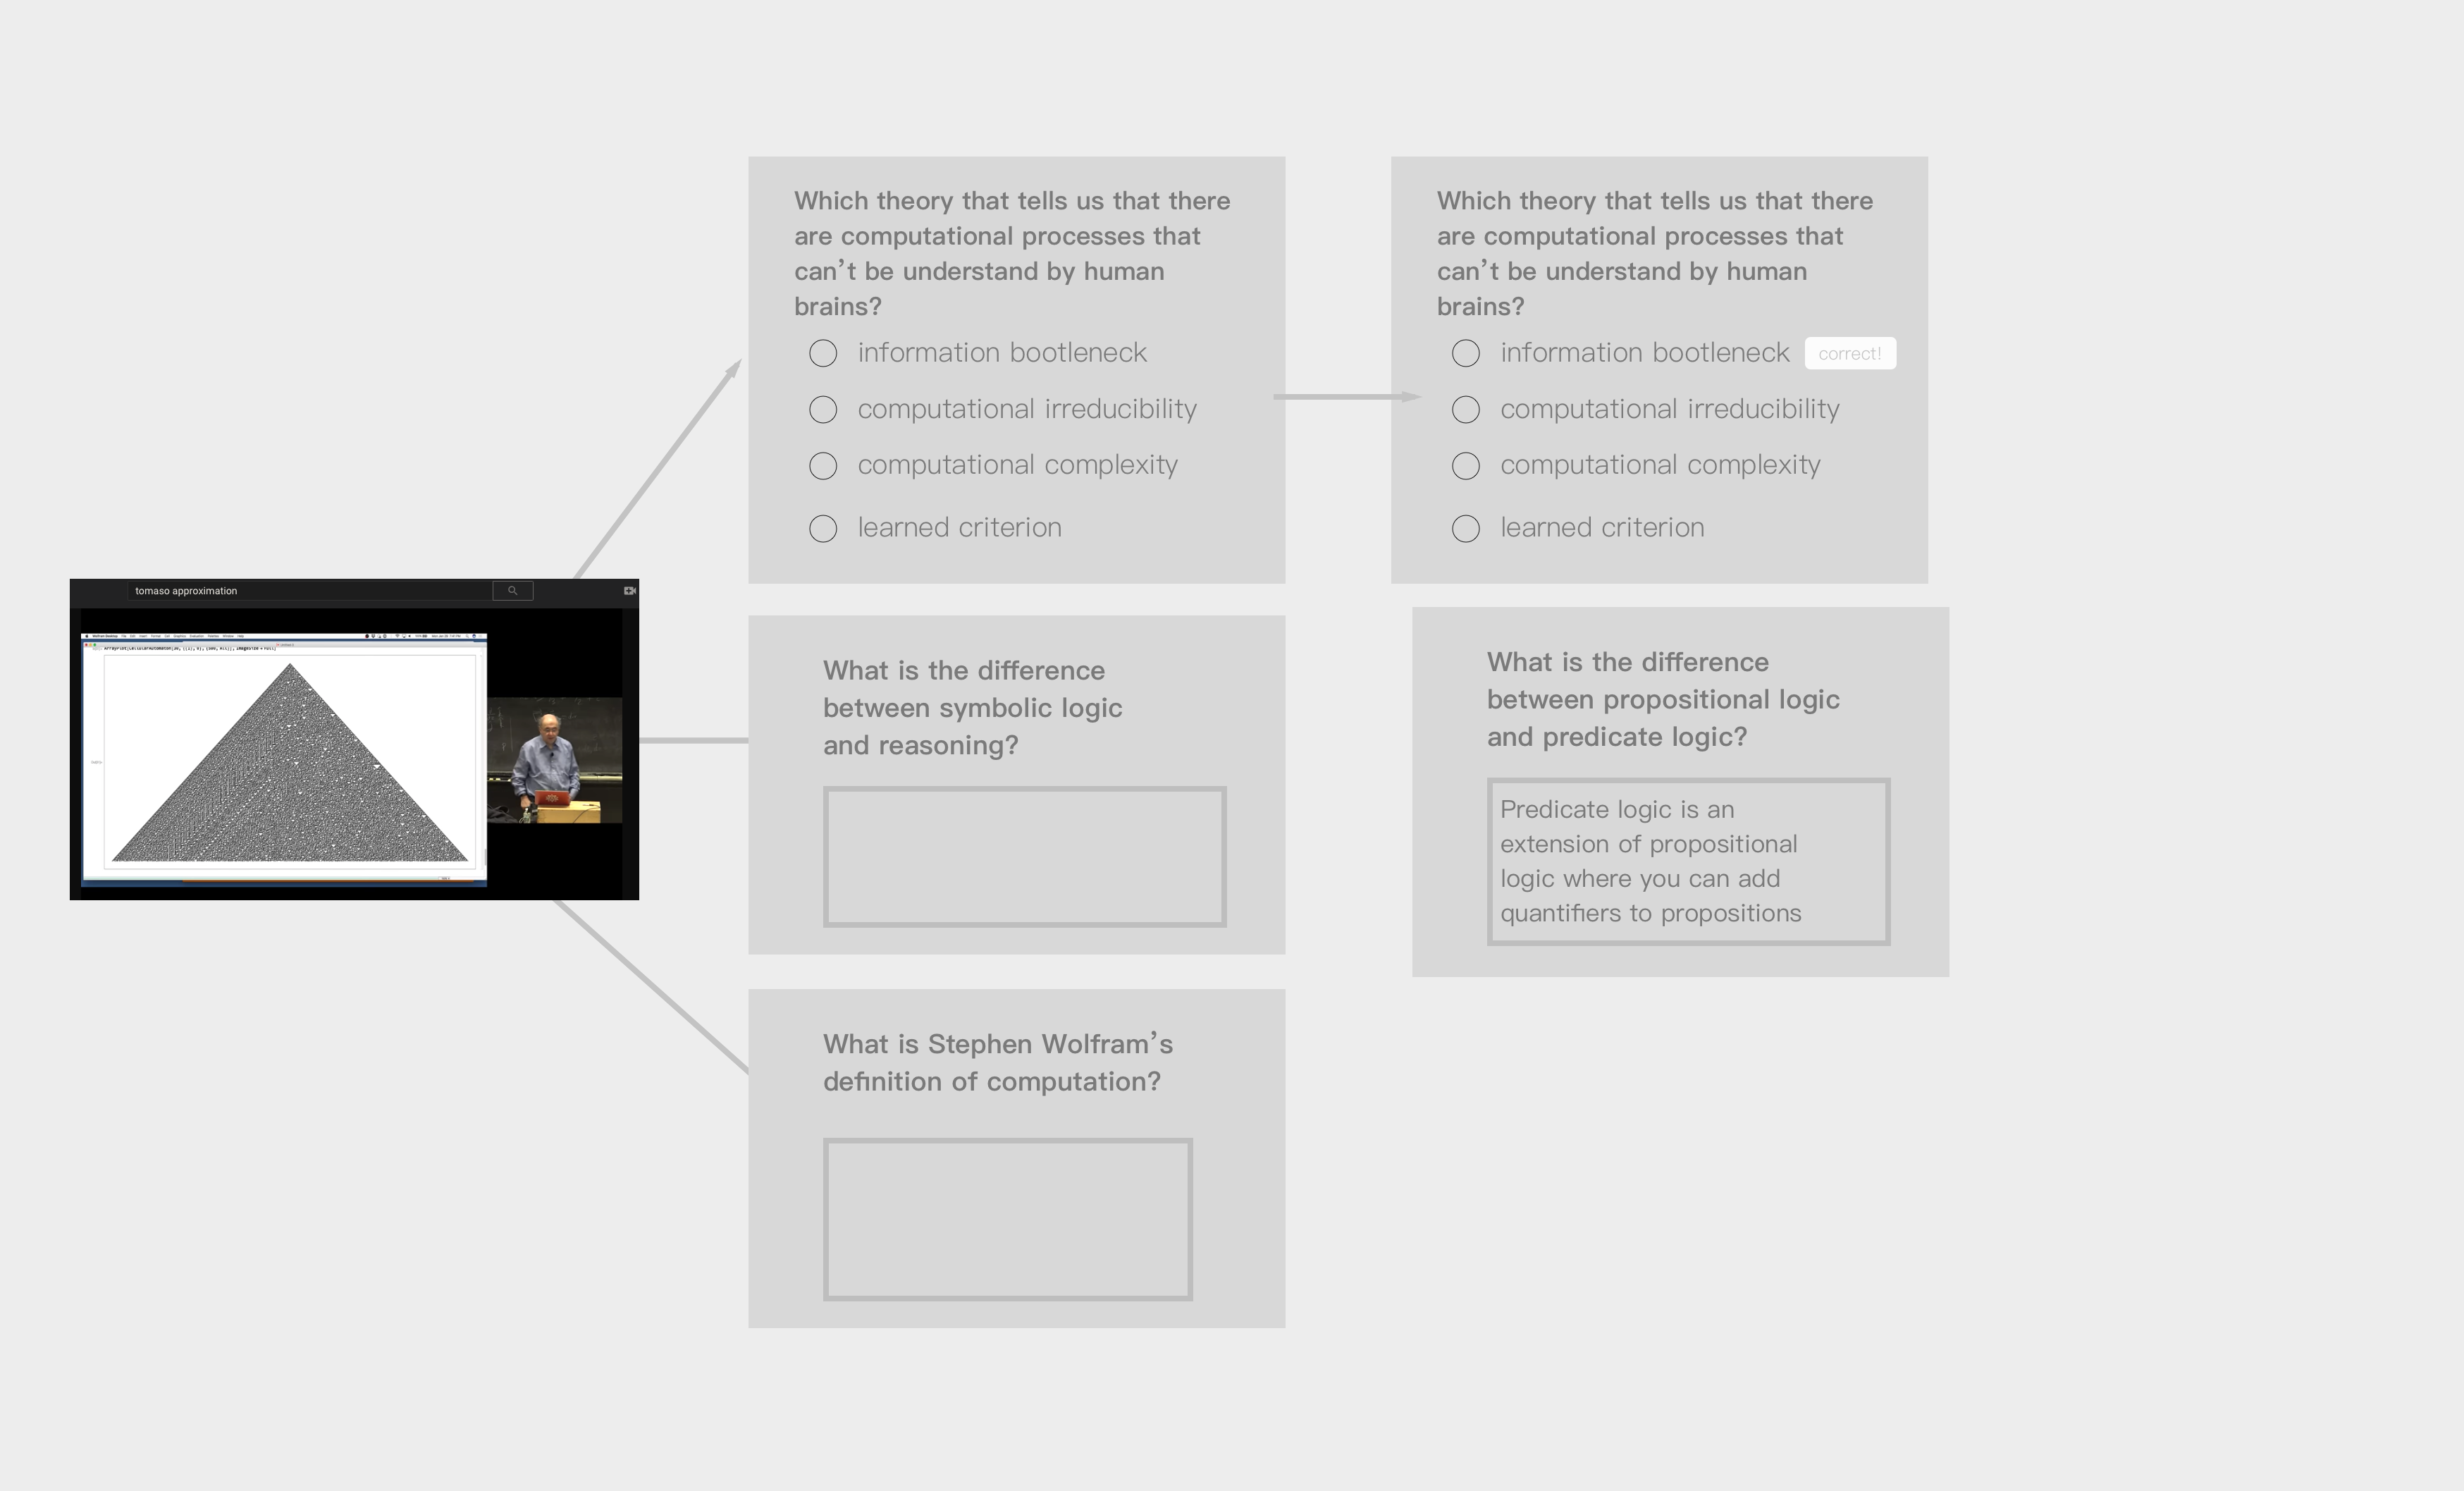
\includegraphics{img/MtoQA.png}
\caption{Image title}
\end{figure}

Let's start with a future view of an individual's education. Many of us
have used the internet to educate ourselves with the abundance of medium
to high quality videos, papers, articles, podcasts and how-tos being
uploaded from numerous individuals, groups, and institutions like never
before (60 hours of video are uploaded to youtube.com every minute).

Let us imagine that all of what you have learned online, throughout the
entirety of your life, from the hundreds of Youtube videos, Wikipedia
articles, Nature papers, and podcasts you've read, watched, or listened
to, were all added structurally to your \textbf{knowledge journey}, and
what if that journey could be consolidated into what we might call a
\textbf{knowledge footprint} that could be shared with others? Could
this replace static degrees? Or augment them to be more inclusive of a
learner's true knowledge? How might we test such knowledge?

Our current approach to education is to treat knowledge acquisition like
a chapter in the individual's life that is limited to one or more formal
places. This is misleading since we accrue knowledge from everywhere and
most recently the internet has become a primary source of knowledge
acquisition but has gone mostly unaccounted for in terms of recognition
(i.e.~watching a whole series of Youtube lectures on the Neurobiology of
Depression or Discrete Mathematics goes mostly unnoticed when someone
views one's resume or by simply looking at their degree.). This makes it
much harder for people to switch to working and exploring outside of
their degree area. Knowing rigourous mathematics and not having a degree
in it, is said to be surprising, therefore the current ``thumbnail
view'' of an individual's knowlede is neccessarily inadequate to the new
mediums of knowledge acquisition.

\begin{figure}
\centering
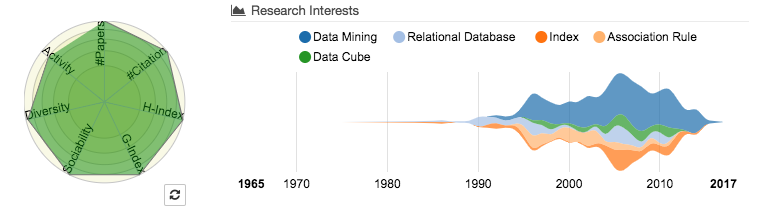
\includegraphics{img/aminer.png}
\caption{Example at aminer}
\end{figure}

The ideas behind this \emph{knowledge ecosystem}, presents only one of
many possible solutions to bringing our education system into modernity.
The goal of it would be to promote the long held idea of the life-long
learner. Moving away from the ``education chapter''" of an individual's
life to the individual as an evolving learner; learning the necessary
skills for what life presents them with today or might tomorrow. It
would (combined with traditional education) show us a more accurate
depiction of a learner's knowledge and theorefore that of a society's
collective knowledge.

Visualised over time, we could begin to capture a learner's so called
\textbf{knowledge journey}. Composed of every piece of content they've
gained knowledge from mapped to the \emph{human knowledge graph}.
Showing how an individual has traversed through the world of human
knowledge.

This would also serve as a way for others, who may be on a similar
\textbf{knowledge journey} to connect with their cohort. This could be
the start of meetups, study groups, and so on.

For those who are looking for a change, they may find different journeys
that help them decide what step to take next. You would also be able to
connect someone's occupation to their \textbf{knowledge journey}.

On aggregate, we could begin to cluster similar \textbf{knowledge
journeys} through unsupervised learning, which might lead to completely
new journeys or combinations of subjects at differnet levels that others
may be inspired to follow.

In this essay, I will propose a \textbf{knowledge ecosystem}, a new way
of approaching education that attempts to build a more accurate
depiction of a learner's true knowledge. It will require significant
effort to bring to life but I believe the benefits will outweigh the
costs. I will talk about how we can use machine learning, deep learning
in particular, to help create and support a \textbf{knowledge ecosystem}
which is made up of a \textbf{knowledge footprint}, \textbf{knowledge
journeys}, and a \textbf{collective human knowledge graph}. We will also
introduce current advances in deep learning that would enable us to take
the space of unstructured educational content on the web and do the
following, - classify content to higher level subjects - map content
unto the human knowledge graph - test a learner's knowledge of recently
viewed educationcal content through questions and answers, no what
matter the subject.

I will also argue that this imagined future is not only
\textbf{desirable} for society but something similar is required to
insure individual's knowledge are well represented in a time where the
pace of change is rapidly speeding up. Let us not forget, that even
software engineering is currently being recreated with machine learning
as a key pillar which wasn't much of a thought 5-10 years ago.

As the future pushes us forward, it is tantamount that we have
adaptative systems that can represent our current knowledge and also
make us predictable to others given the future pushes us to knowing more
than ever and knowing who to collaborate with to apply such knowledge.

This hypothetical future isn't just conceptual, most of what I will
present to you today is currently feasible due to the most recent
advances in machine learning, and in particular deep learning

In the last section of this essay I will review what has been proposed
and also call other researchers, teachers, and designers to collaborate
on such an ecosystem, even if it is just in part.

*For the purpose of this essay we will talk mostly about digital
knowledge acquisition and leave the reader to extend the basics to
knowledge obtained elsewhere.

\chapter{Primary Concerns}\label{primary-concerns}

There are 3 popular concerns that I will attempt to address in this
article about online knowledge acquisition that stand in the way of
having an adaptive and reliable knowledge ecosystem. I will attempt to
present a system that can sufficiently overcome each of the concerns
here and in the implementation section.

There are as follows:

\begin{itemize}
\tightlist
\item
  \textbf{Passive Consumption} - most of online content is viewed
  passively by the learner and the result of passive consumption is that
  learner's do not grasp the concepts or master the content being
  taught.
\item
  \textbf{Untested Knowledge} - even if the learner was engaged while
  viewing a piece of educational content their knowledge is untested and
  therefore it isn't clear if they've mastered the content accurately
  and in some sense holistically.
\item
  \textbf{Knowledge Representation} - even if the learner was engaged
  (1) and their knowledge was tested (2), simply knowing the counts or
  types of video they watched doesn't make their knowledge predictable
  and useful to others. In fact, even the learner may be unaware of all
  of what they've viewed.
\end{itemize}

\section{Passive Consumption and Untested
Knowledge}\label{passive-consumption-and-untested-knowledge}

\begin{quote}
How would such an ecosystem insure us against passive consumption?
\end{quote}

Scenario \#1: A learner goes online and begins watching a series on
Machine Learning. How do we engage and test a user's knowledge?

Proposition: Using advances in deep learning, we propose a dual question
and answer generation given the educational content.

Result: A learner gets a set of questions and multiple choice answers
throughout the video. Keeping the user engaged and sharp to ensure they
can answer each of the questions.

As you can see, I've bundled passive consumption and untested knowledge
because our proposed ecosystem approaches both of these by always
testing knowledge. I will show the current results in deep learning in
the implementation stage.

\section{Knowledge Ecosystem Example}\label{knowledge-ecosystem-example}

\begin{figure}
\centering
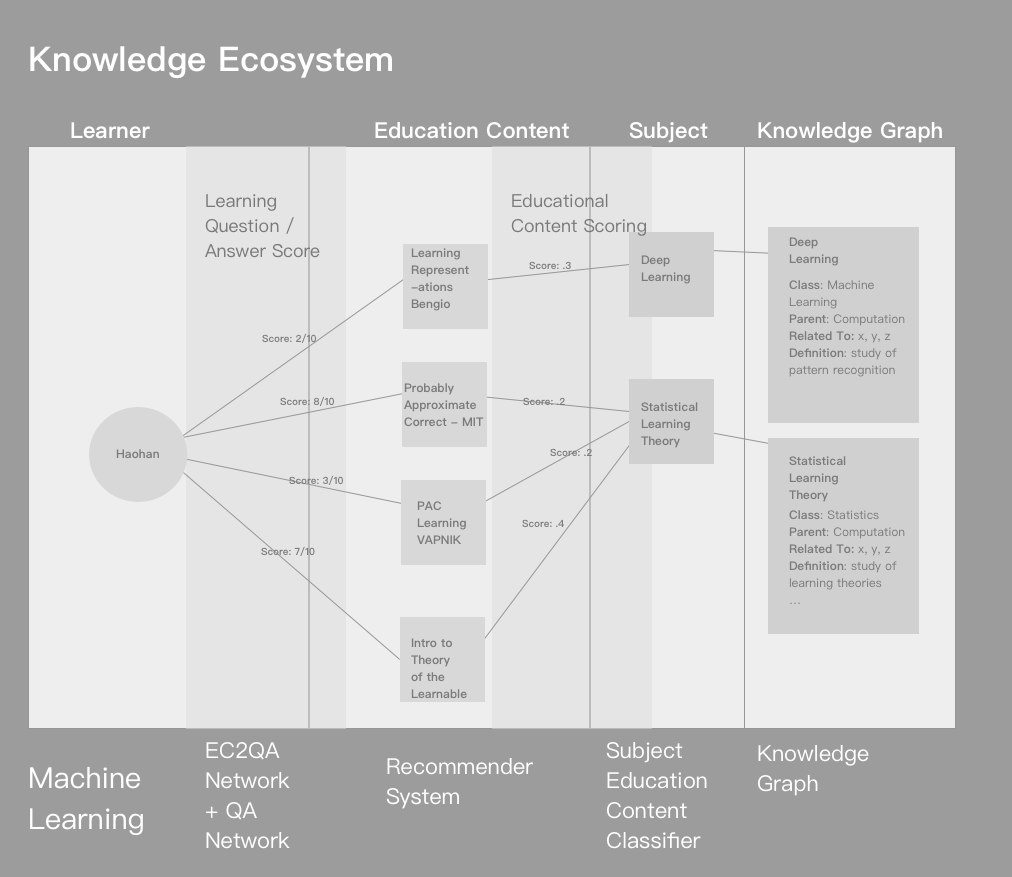
\includegraphics{img/knowledgeEcosystem.png}
\caption{Knowledge Ecosystem}
\end{figure}

Given a piece of educational content, our knowledge system will generate
a set of questions and answers that theoretically capture the major
concepts and facts that the learner should know after viewing a part or
the content in whole.

You can imagine watching a Youtube video and after a learner views 15
minutes of an hour long lecture on computational complexity a quiz is
presented (a set of questions and answers conditioned on the past 15
minutes of video,) and the results are recorded. In the future we would
also be able to use the knowledge graph

The knowledge system would only consider content that has been watched
with some engagement or if they can test out of the content.

\section{The Problem of Knowledge
Representation}\label{the-problem-of-knowledge-representation}

\begin{quote}
Given how many learner's online knowledge acquisition varies and has
been invisible up to now, how we can best represent their knowledge?
\end{quote}

Scenario \#2: A learner has a degree in Public Health, but since
graduating, they've been studying machine learning for the last 3 years.
The learner now wants to apply to a job that requires Health and
Statistics. How do we represent their traditional and updated knowledge?

This is a tricky problem that goes beyond any given algorithm. The exact
design of a \textbf{knowledge footprint} and a \textbf{knowledge
journey} has been attempted and we will not cover that in depth here.
The proposed system presupposed the design of the knowledge footprint.

There are two problems, \textgreater{} how do we reduce someone's
knowledge (in this case a set of educational content and their
respective scores) into a symbol

Proposition: We introduce \textbf{knowledge journeys} and the
\textbf{knowledge graph} as a way to make sense and structure a
learner's knowledge acquisition. The collective \textbf{knowledge graph}
will tell us about the subject the learner is studying and we can use
this to compare to others and create a relative comparison.

Result: Reducing a learner's \textbf{knowledge journey} into a common
set of elements that makeup into their \textbf{knowledge footprint}
which would look similar to those with similar journeys.

So the employeer, now familiar with the footprints can see the overlap
between the current employee's and a prospective employee.

\chapter{Concepts}\label{concepts}

\section{Knowledge Footprint}\label{knowledge-footprint}

The concept of a knowledge footprint is a custom symbol or badge with a
profile that represents one's education relative to that of others. This
footprint should represent all of one's education (currently focused on
digital) while balancing distinction and commonality with others.

This example from aminer is very helpful.
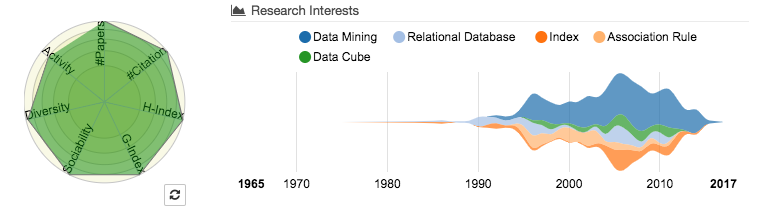
\includegraphics{img/aminer.png}

\section{Knowledge Journeys}\label{knowledge-journeys}

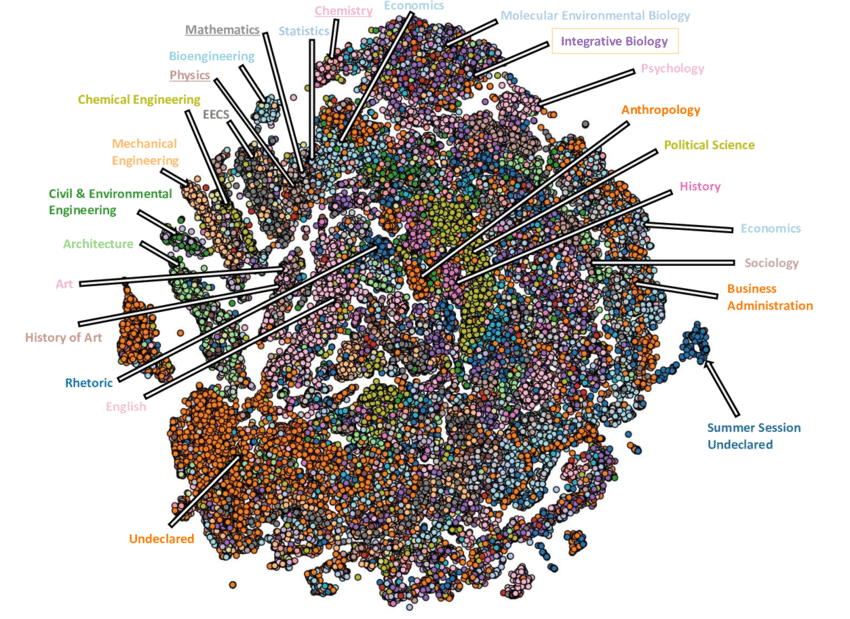
\includegraphics{img/tsne.png} Image src:
\url{https://www.researchgate.net/figure/t-SNE-projection-of-the-embedding-of-all-learners-in-the-dataset-Major-labels-are_fig1_323391033}

A \textbf{knowledge journey} is a somewhat simplified view of all of the
educational content a learner has acquired over time. The journey should
be a temporal representation of all of the subjects that one has viewed
and been tested on. Knowledge journey's should be simple enough to
compare but complex enough that the individual can go back to a
particular moment in time and rewatch educationcal content they've
viewed before.

\section{Collective Human Knowledge
Graph}\label{collective-human-knowledge-graph}

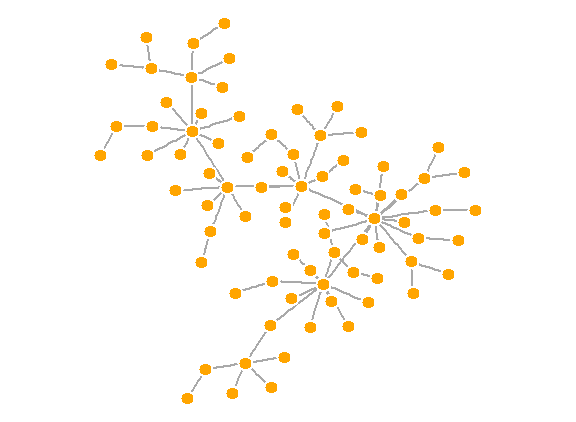
\includegraphics{img/knowledge_graphy.png} The collective human
knowledge graph can be compared to Google's Search Knowledge Graph which
points unstructured information towards structure. The graph should have
all existing subjects that we are currently aware of (i.e.~Abstract
Mathematics, Discrete Mathematics, Statistics, Art, Sociology). Since
each piece of educational content will be classified into a subject, all
subjects will exist in detail within the knowledge graph.

\subsection{EC2QA Network}\label{ec2qa-network}

We mentioned the EC2QA network earlier because currently we would have
to cobble together multiple networks to make this work. Instead we will
introduce a novel network architecture, EC2QA, to solve the problem of
generating a set of questions and answer pairs for any given educational
content (text, video, image, pdf).

\section{Knowledge Ecosystem
Example}\label{knowledge-ecosystem-example-1}

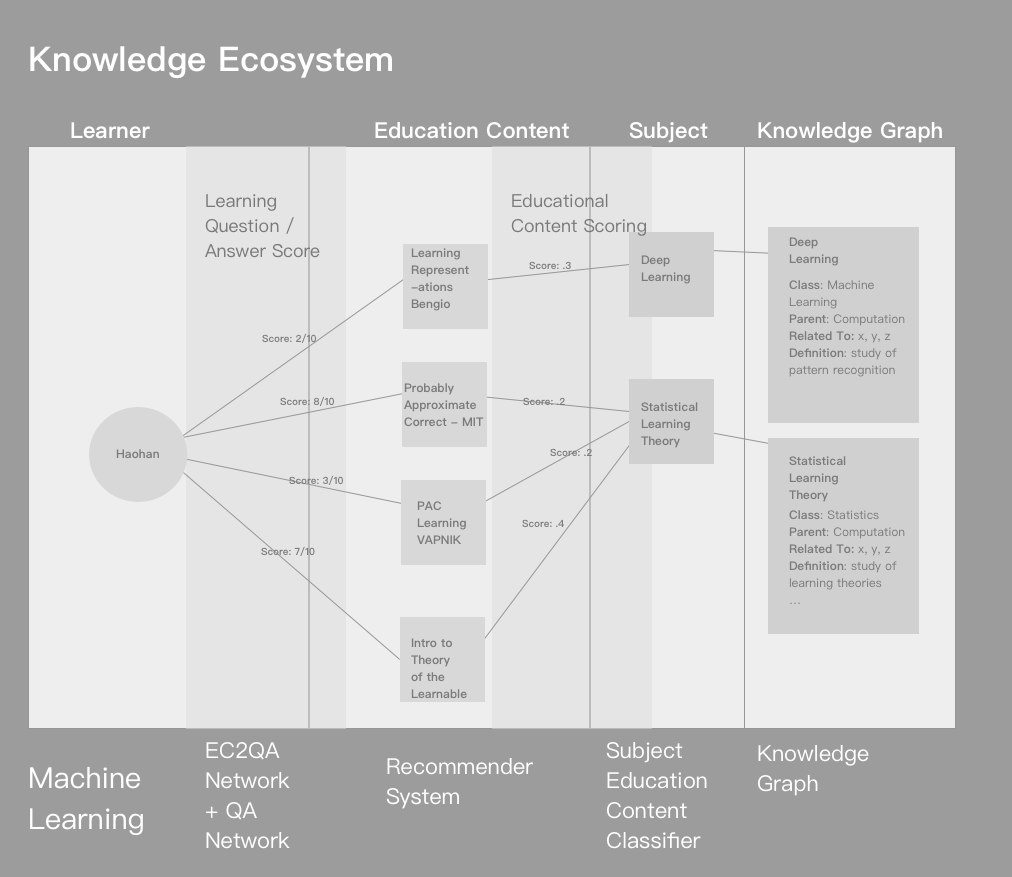
\includegraphics{img/knowledgeEcosystem.png} Now that we are aware of
each of the elements, let's talk about how they work in practice.

A learner watches a video titled `Depression' by Robert Sapolsky. - The
video is classified by a neural network as {[}Neuroscience, Mental
Health, Psychology{]} - The subjects are then mapped to the
\textbf{knowledge graph} which gives us more information about each
subject - Using EC2QA or similar, a set of questions and answers are
generated for every 15* minutes of video A learner is present with 5
questions to answer and scores 4/5 (80\%) - The link between user and
video takes up the score At the end of the video, the learner records a
video summary and is evaluated with a 7/10 (70\%) - The evaluation
network looks at the \textbf{semantic and conceptual mututal
information} shared between the original content and the learner's video
summary - All scores are mapped to the video and also counted at the
subject level A learner looks at their knowledge footprint - All scores
should be calculated against all subjects coming from the knowledge
graph and compared against other learners to generate the footprint

\chapter{Implementing the Knowledge
Ecosystem}\label{implementing-the-knowledge-ecosystem}

In this section, we are set to solve the following question:

\begin{quote}
How might we approach designing such a system.
\end{quote}

In this section, we will walk you through some possible implementations
of the proposed knowledge ecosystem. We will be presenting the current
research in machine learning that is relevant to each component of the
knowledge ecosystem while aslo discussing this new artificial neural
network architecture EC2VQA and one possible instansitation of that.

Note that this is not the blueprint, each of these components can be
developed independently and vary from what you find here. This is a
provocation for getting started on the knowledge ecosystem today.

\section{Problem Formulation}\label{problem-formulation}

Building such a knowledge ecosystem is not a trivial task. An necessary
step of searching for the proper solutions would be trying to break the
whole task into few subtasks that we can deal with separately. As what
we have discussed earlier, our ecosystem could be divided into few key
building blocks as below:

\begin{enumerate}
\def\labelenumi{\arabic{enumi}.}
\item
  \textbf{Learning + Feedback} -- given a learner consumes a piece of
  educational content, reliably evaluate their knowledge and provide the
  feedback for improvement to support their learning. (credibility,
  rigour)
\item
  \textbf{Knowledge Graph} -- general knowledge blueprint as a map to
  piece together all the content that is currently available.
  (relatibility, predictability)
\item
  \textbf{Knowledge Journeys} -- given a piece of educational content,
  classify it within a knowledge graph; given multiple learner journeys,
  create a way to customize their own growth journey while offereing a
  way for them them to compare, connect with and follow, other's journey
  (compare, traverse, curiosity)
\item
  \textbf{Knowledge Footprint} -- given a learner's journey, collapse it
  into a representative symbol(s) (digital education footprint)
  (relatibility, stable but evolving system )
\end{enumerate}

Much of the element \#1 and \#2 have been made possible with the recent
breakthoughs in machine learning especially in the filed of deep
learning. A few other pieces like the element \#3 and \#4 may require a
more advanced framework that has not been proposed yet to best resolve.
Let's first take a look at some methods that might come handy when
applying to our problems.

In this section we will be primarily focus on the first 2 building
blocks.

\subsection{Before we start\ldots{}}\label{before-we-start}

As what we discussed above, one of the possible and optimal solutions so
far for building our ecosystem is using current state-of-art tehcniques
i.e.~deep learning in the related domains. Here I will walk you through
some thought provoking research summary in a form of survey.

To best illustrate the problem and possible solutions, we will for now
reduce the complexity of the problem. As what we have mentioned earlier,
educational videos seem to be one of the top options for people when it
comes to knowledge acquisition. Keep in mind that our ultimate goal is
to be able to apply our system to any type of online available
educational content.

Let's explore some of the solutions that can enable us to apply our
system on the video educational content.

\section{Learning + Feedback}\label{learning-feedback}

\subsection{Question Formulation}\label{question-formulation}

We consider learning + feedback as a key building block of the ecosystem
which is the cure for our primary concern of passive knowledge
consumption and untested knowledge of learners. By solving this problem,
our system will be able to provide our learners a credible and
interactive learning experience that can best support their knowledge
acuqisition.

In shor, in the section we will be providing some insights on how to
solve the following puzzle:

\begin{quote}
``how can we take a piece of educational content and properly test a
learners' knowledge and provide insightful feedbacks to support their
learning?''.
\end{quote}

\subsection{Dive into the solutions}\label{dive-into-the-solutions}

In previous years, deep learning research has taken up a similar problem
titled Question Generation (QG) and Question Answering (QA).

Question Generation (QG) is part of NLP. The goal of QG is to generate
questions according to some given information. It could be used in many
different scenarios i.e.~generating questions for reading comprehension,
generating data from large scale question-answering pairs or even
generating questions from images. Earlier approaches to QG mainly used
human-crafted rules and patterns to transform a descriptive sentence to
a related question. Recent neural network-based approaches represent the
state-of-art of most of those tasks and this approach has been
successfully applied to many other NLP tasks i.e.~neural machine
translation, summarization, etc. As the training optimization studies
progress, the stability and performance improvements are gauranteed.

As for Question Answering (QA) task, it is a well-researched problem in
NLP as well. Recently, QA has also been used to develop dialog systems
and chatbots designed to simulate human conversation. Traditionally,
most of the research used a pipeline of conventional
linguistically-based NLP techniques i.e.~parsing, part-of-speech tagging
and coreference resolution. However, with recent developments in deep
learning, neural network models have shown promise for QA. Further
improvement i.e.attention mechanism and memory networks allow the
network to focus on the most revevant facts such that they achieved
state-of-art performance for QA.

Now we have some basic understanding of these 2 problems for which we
will be expanding more in depth later. Consider the next question:

\begin{quote}
``what types of questions \& answers would be best to test a learner's
knowledge given a piece of educational content (i.e.~a lecture video)''
\end{quote}

Let's say a learner is watching a video about hypothesis testing, after
showing an example and giving the data needed to test the hypothesis.
The system could pause the video and ask the following possible
questions:

\begin{enumerate}
\def\labelenumi{\arabic{enumi}.}
\item
  What is the p-value for this test? (and provide multiple choices for
  learner to choose from)
\item
  Is this a 1-sided test? (answers provided would be: YES or NO)
\item
  How would you intepret the p-value in the context of this example.
\item
  Based on your calculation, summarize the conclusion of this hypothesis
  testing for me.
\end{enumerate}

It is also helpful to ask learner the question as follows after showing
the solution:

\begin{enumerate}
\def\labelenumi{\arabic{enumi}.}
\setcounter{enumi}{4}
\tightlist
\item
  Tell me what you have learned through this video or this example.
\end{enumerate}

As shown above, we would call questions \#1 and \#2 the close-ended
questions; question \#3 and \#4 the specific open-ended questions; and
question \#5 a general open-ended question.

Based the above information, we can update our question formulation
into:

\begin{enumerate}
\def\labelenumi{\arabic{enumi}.}
\item
  Generate close-ended question + answers pairs
\item
  Generate specific open-ended question + answers pairs
\item
  Evaluate and comment on the general open-ended answers
\end{enumerate}

In terms of the close-ended, the answers can be well defined and
evaluated. However, the process might be a little bit tricky when it
comes to the open-ended questions. We will approach each of them here
from the current research perspective.

** Why deep learning? **

As we stated above, deep learning has achieved state-of-art performance
in both QG and QA tasks. But how?

If you pay close attention to the question generation and answer
generation type of problems, you can easily reframe this problem into a
general machine learning problem in which the model needs to learn the
relationship between the educational content and the meaningful question
\& answer pairs that is associated with the content. In other words, our
problem could be simplified as learning a function that is capable of
capture the relationship between our input and output, or, appropriately
map the educational content to the desired question and answer pairs
with this function.

To the best of our knowledge, deep learning is one of the most optimal
techniques currently developed to do such a job

As we all know that machine learninag is a set of algorithms that can be
used to parse data, learn from the data, and then apply what they have
learned to make intelligent decisions. Or more specifically, deep
learning is a subset of machine learning that belongs to the family of
representation learning. Inside this family, deep learning is
particularly good at sampling the features and having additonal layers
for more abstract feature learning. All of these features are crutial
for our goal of mapping the feature to the output task.

Because of the above advantages, deep learning is known as one of the
most flexible machine learning algorithms that can learn and map the
\textbf{deep representation} from the data. Also, deep nueral networks
architecture can be composed into a single differentiable function and
trained end-to-end until it converges. As a result, they can help
identify the suitable \emph{inductive} \emph{biases} catered to the
training data.

Moreover, deep learning outperforms other techniques when the training
data size is large and the advantage fits our siutation well. We could
easily find a large amound of educational content available on the web.

The large amount content creates another problem that can be avoided
with deep learning, which is it's going to be very troublesome if you
plan to do feature engineering manually. When there is lack of domain
understanding for feature introspection, deep learning is preferable.

In the end, deep learning really shines when it comes to many complex
reserach problems such as NLP, Visual Recognition and Speech
recognition. For solving our task, all those domians will possibly be
invloved.

\subsection{Question Generation}\label{question-generation}

Let's begin with question generation (QG) problem.

The ideal goal of an automatic question generation is to generate a
question Q that is syntactically and semantically correct, relevant to
the context and meaningful to answer.

In order to achieve this goal,, we need to train an algorithm to learn
the underlying conditional probability distribution \[P_{\theta}(Q|X)\]
parametrized by \(\theta\). In other words, we can think of this problem
as the one that requires the model to learn a function (with a set of
parameters) \(\theta\) during the training stage using content-question
and/or answer pairs so that the probability \(P_{\theta}(Q|P)\) is
maximized over the given training dataset.

It is also helpful to frame this problem into a seq2seq learning problem
since both the input and the output are most likely a sequence of text
character that the model needs to process and learn the relationship
from.

\subsubsection{Case Studies}\label{case-studies}

\begin{enumerate}
\def\labelenumi{\arabic{enumi}.}
\tightlist
\item
  In this paper
  \href{http://www.princeton.edu/~shitingl/papers/18l@s-qgen.pdf}{QG-Net:
  A Data-Driven Question Generation Model for Educational Content}. They
  use a bi-directional LSTM network to process the input context words
  sequence. Encoding the answer into context word vectors.
\end{enumerate}

QG-Net generates questions by iteratively sampling question words from
the conditional probability distribution \(P(Q|C,A,\theta)\) where
\(\theta\) denotes the set of parameters. In order to construct the
probability distribution, they first create a \textbf{context reader}
that process each word \(c_j\) in the input context and turns it into a
fix-sized representation \(h_j\)

Then, they used a \textbf{question generator} generates the question
text word-by-word, given all context word representation and all
question words in previous time steps.

As for the quantitative evaluation, they aimed to minimize the
difference between the generated question and the true question in the
training set during training. Also, they used the standard
back-propagation through time with the mini-batch stochastic gradient
descent algorithm to learn the model parameters. They employed teacher
forcing procedure for training LSTMs. To enhance performance, they also
implemented beam search, a greedy but effective approximation to
exhausitively search and select the top 25 cancidate output question
sentences. The final one would be the one with the lowest negative log
likelihood.

The general QG-Net model Architecture is as below:

\begin{figure}
\centering
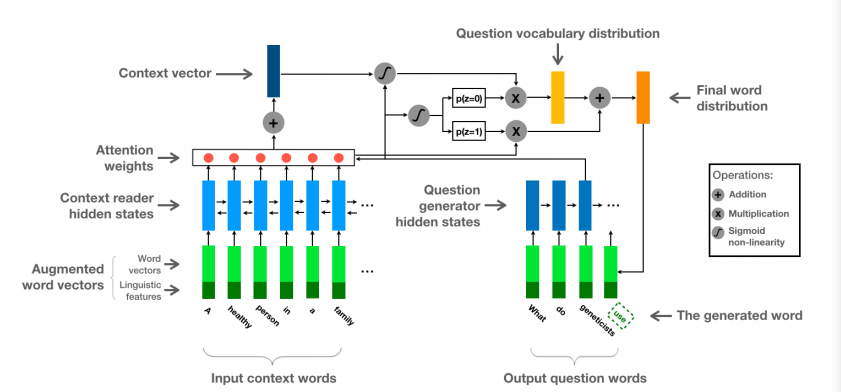
\includegraphics{img/qgnet.png}
\caption{ma}
\end{figure}

\begin{enumerate}
\def\labelenumi{\arabic{enumi}.}
\setcounter{enumi}{1}
\tightlist
\item
  In this summary
  \href{http://www.cs.cornell.edu/~xdu/papers/acl17_dsc_poster.pdf}{Learning
  to Ask}, they used a sentence- and paragraph-level seq2seq model to
  read text from the input content and to generate a question about the
  input sentence.
\end{enumerate}

For the second option, we need to encode both sentence and paragraph
that sentence belongs to as input, but only attending source sentence
hidden states. The performance could be improved with beam search and
UNK replacement.

\begin{enumerate}
\def\labelenumi{\arabic{enumi}.}
\setcounter{enumi}{2}
\tightlist
\item
  In this paper
  \href{https://openreview.net/pdf?id=rk3pnae0b}{TOPIC-BASED QUESTION
  GENERATION}, they proposed a topic-based question generation
  algorithm. The algorithm will be able to take in a input sentence, a
  topic and a question type; then generate a word sequence related to
  the topic, question type and the input sentence.
\end{enumerate}

They are formulating a conditional likelihood objective function to
achieve this goal.

Also, in the paper, they proposed a few frameworks that were used to
tackle this problem. The first type is seq2seq model. This model
typically uses a bidirectional LSTM as the encoder to encode a sentence
and a LSTM as the decoder to generate the target question.

The second approach is question pattern prediction and question topic
selection algorithms. It takes in an automatically selected phrase Q and
fill this phrase into the pattern that was predicted from pre-mined
patterns, which is not done with deep learning.

The last approach is multi-source seq2seq learning which aims to
integrate information from multiple sources to boost learning.

\begin{enumerate}
\def\labelenumi{\arabic{enumi}.}
\setcounter{enumi}{3}
\tightlist
\item
  In this paper \href{https://arxiv.org/pdf/1808.04961.pdf}{A Framework
  for Automatic Question Generation from Text using Deep Reinforcement
  Learning} they proposed a novel way of solving this problem in which
  they used a reinforcement learning framework that consists of a
  generator and an evaluator.
\end{enumerate}

They refer to the generator as the \(agent\) and the \(action\) of the
agent is to generate the next work in the question. The probability of
decoding a word \(P_{\theta}(word)\) gives a stochastic policy.

The evaluator will in turn assign a reward for the output sequence
predicted using the current policy of the generator. Based on the reward
assigned by the evaluator, the generator updates and improves its
current policy. The goal in RL-based question generation is to find a
policy that can maximize the sum of the expected return at the end of
the sequence generated.

\subsubsection{Summary}\label{summary}

In this QG section, we have discussed 4 algorithms. They provide us a
way to frame our problem for which we can apply generative seq2seq model
framework. As for our objective function, we are formuating a
conditional probability distribution that is conditioned on the provided
content (i.e.~the video) and answers. Typically, we can use a
bi-directional LSTM as the encoder to encode the content and use a LSTM
as the decoder to generate the question.

However, as you probabily have noticed that the above examples are focus
mainly on processing the text input data instead of videos directly. It
demonstrates that more reserch in this new area is needed so as to meet
our particular needs.

\subsection{Answer Generation}\label{answer-generation}

\subsubsection{Close-ended Questions}\label{close-ended-questions}

\paragraph{Visual Question Answering
(VQA)}\label{visual-question-answering-vqa}

As what we have covered above, most QG problem focuses solely on
generating questions but not the answers based on the context.

VQA is a challenging research problem that focuses on providing a
natural language answer given any image and any free-form natural
language question. As we are managing to handle the video educational
content first that is likely to involve language processing and visual
recognition tasks, VQA would be a proper start for us. By leveraging
this type of algorithm, we enable our system to easily evaluate the
answer provided by learners which could in turn automated the whole
question + answering + evaluation cycle.

Since we are dealing with visual input, question-guided attention
mechanism is a key component for solving this type of task. Started from
the attention mechanism that can adaptively learn the most relevant
image regions for a given question. Then to stack multiple
question-guided attention mechanisms to learn the attention in an
iterative way. Also, it is possible to use bilinear features to
integrate the visual features from the image spatial grids with question
features to predict attention. Considering the questions in natural
language may also contain some noise, the co-attention mechanism can
jointly learn the attention for both the image and question.

\subparagraph{Case Studies}\label{case-studies-1}

\begin{enumerate}
\def\labelenumi{\arabic{enumi}.}
\tightlist
\item
  In this paper
  \href{http://openaccess.thecvf.com/content_ECCV_2018/papers/Yalong_Bai_Deep_Attention_Neural_ECCV_2018_paper.pdf}{Deep
  Attention Neural Tensor Network for Visual Question Answering}, they
  proposed a novel deep attention neural tensor network that can
  discover the joint correlation over images, questions and answers with
  tensor-based representation.
\end{enumerate}

As for their workflow, they modeled one of the pairwise interaction
(i.e.~between image and question) by bilinear features, which is further
encoded with the thrid dimension (i.e.~answer) to be a triplet using
bilinear tensor product. During this step, the model takes in a question
+ a corresponding image + candidate answers as the input. A CNN
(convolutional neural network) a GRU RNN (recurrent neural network) are
used for extracting feature vectors and question respectively. Then the
representation is passed on as a multi-modal features and integrated by
bilinear pooling module. Moreover, they decompose the correlation of
triplets by their question and answer types with a slice-wise attention
module on tensor to select the most discriminative reasoning process
inference.

In the end, they optimize the proposed network by learning a label
regression with KL-divergence losses.

They clamined that with these techniques, they can enable scalable
training and fast convergence over a large number of answer set.

During the inference stage, they feed the embeddings of all candicate
answer into the network and then select the answer which has the biggest
triplet relevance socre as the final answer.

The high-level network architecture is as follows:

\begin{figure}
\centering
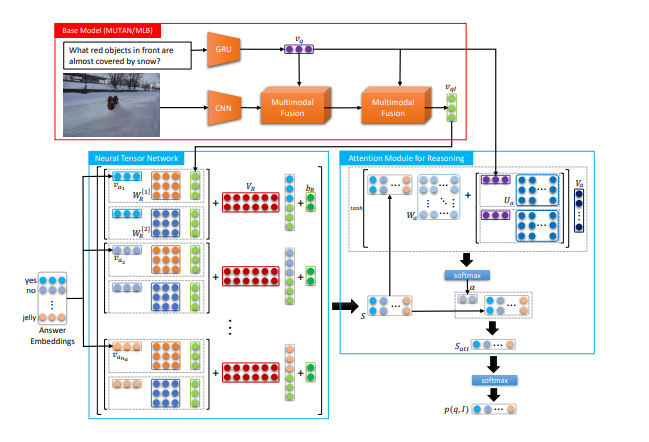
\includegraphics{img/vqa.png}
\caption{Deep Attention Neural Tensor Network}
\end{figure}

\begin{enumerate}
\def\labelenumi{\arabic{enumi}.}
\setcounter{enumi}{1}
\tightlist
\item
  In this paper \href{https://arxiv.org/pdf/1804.02088.pdf}{Question
  Type Guided Attention in Visual Question Answering}, they proposed a
  model called Question Type-guided Attention (QTA). This model utilizes
  the information of question type to dynamically balance visual
  features from both top-down and bottom-up orders.
\end{enumerate}

Finally, they propose a multi-task extension that is trained to predict
question types from the lexical inputs during training which generalizes
the network into applications that lack question type, with a minimal
performance loss.

As for their main contribution, they focus on developing an attention
mechanism that can exploit high-level semantic information on the
question type to guide the visual encoding process.

Specifically, they introduced a novel VQA architecture that can
dynamically gate the contribution of ResNet and Faster R-CNN features
based on the question type. In turn, it allows them to integrate the
information from multiple visual sources and obtain gains across all
question types.

\paragraph{Video Question Answering}\label{video-question-answering}

The recent advancements that we discussed above in VQA domain have shown
some promising implication. In terms of achieving our particular goal,
it is also worth mentioning that VQA might be a good start but it is not
sufficient yet. To bridge this gap, let's focus our attention on some
video question answering algorithms that have been proposed.

\subparagraph{Case Studies}\label{case-studies-2}

\begin{enumerate}
\def\labelenumi{\arabic{enumi}.}
\tightlist
\item
  In this paper
  \href{https://www.ijcai.org/proceedings/2018/0513.pdf}{Multi-Turn
  Video Question Answering via Multi-Stream Hierarchical Attention
  Context Network}, they proposed a hierarchical attention context
  network for context-aware question understanding by modeling the
  hierarchically sequential conversation context structure. They also
  incorporate the multi-step reasoning process fro the multi-stream
  hierarchical attention context network to enable the progressive joint
  representation learning of the multi-stream attentional video and
  context-aware question embedding.
\end{enumerate}

The construct their dataset by collecting the conversational video
question answering datasets from YouTubeClips and TACoS-MultiLevel in
which the first one has 1987 videos and the second daaset has 1303
videos. They invite 5 pairs of crowd-sourcing workers to construct 5
different conversational dialogs. In total, they have collected 37228
video question answering pairs for TACoS-MultiLevel data and 66806 ones
for YouTubeClips data.

\begin{enumerate}
\def\labelenumi{\arabic{enumi}.}
\setcounter{enumi}{1}
\tightlist
\item
  In this paper \href{https://arxiv.org/pdf/1512.02902.pdf}{MovieQA:
  Understanding Stories in Movies through Question-Answering}, they
  introduced a new dataset called MovieQA dataset that can evaluate
  automatic story comprehension from both video and text.
\end{enumerate}

They collected 408 subtitled movies and obtained their extended
summaries in the form of plot synopses(movie summaries that fans write
after watching the movie) from Wikipedia. They used plot synopses as a
proxy for the movie. They have annotators create both quizzes and
answers pairs by referring to the story plot. Time-stamp is also
attached with each question.

In the second step of data collection, they used the multiple-choice
answers and question collected as the input to show to the annotators.
By doing so, annotators can re-formulate the question and answers while
doing the sanity check.

\paragraph{Summary}\label{summary-1}

By going through the previous examples, we can see that VQA is very
particular type of algorithms that is designed to efficiently process
image and text input data while making the inference based on the input.
Attention is a typical mechanism applied in this type of problems and
multiple forms of multipulation on the attention mechanism used in these
models have significantly improved the model performance.

Going from VQA to video question answering algorithm, it has been a
great leap. The main insight we can directly draw from these video QA
papers is that we can follow their steps to collect and annonate our
training data by asking crowd-sourcing workers to construct the question
and answer pairs. Also, more advanced algorithm like the one described
above multi-stream hierarchical attention context network is in need for
dealing with video input data in contrast to static pictures.

\paragraph{Dual Question-Answering
Model}\label{dual-question-answering-model}

Both Question Generaion(QG) and Question Answering(QA) are well-defined
2 sets of models that aim to either infer a question or an answer given
the counterpart based on the context. However, they are usually explored
separately despite of their intrinsic complementary relationship. In our
case, a sysem that can take on both roles simultaneously are needed to
fully automated learning + feedback process.

There are some algorithms are designed to fulfill both roles.

\subparagraph{Case Studies}\label{case-studies-3}

1.In this paper \href{https://arxiv.org/pdf/1809.01997.pdf}{Dual
Ask-Answer Network for Machine Reading Comprehension} they presente a
model that can learn question answering and question generation
simultaneousely. They tie the network components that playing the
similar roles into 2 tasks to transfer cross-task knowledge during
training. Then the cross-modal interaction of question, context and
answer is captured with a pair of symmetric hierarchical attenion
processes.

The high-level architecture of the model is illustrate as below:

\begin{figure}
\centering
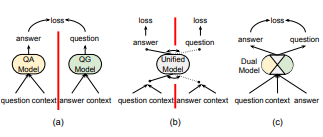
\includegraphics{img/qgqa.png}
\caption{Dual Ask-Answer Network 1}
\end{figure}

\begin{figure}
\centering
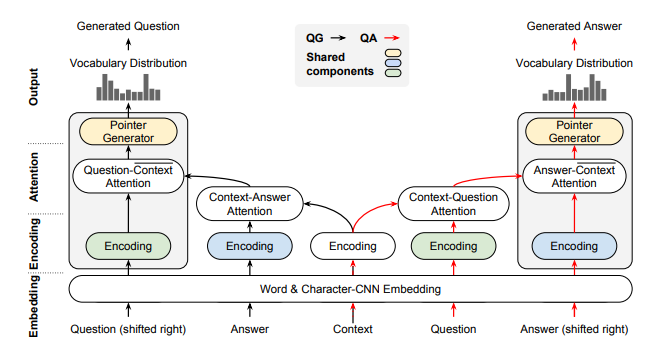
\includegraphics{img/daan.png}
\caption{Dual Ask-Answer Network 2}
\end{figure}

In short, the model is composed of embedding layer, encoding layer,
attention layer and output layer. The model is fed with a
question-context-answer triplet (Q,C,A) and the decoded Q and A from the
output layer. Their loss function consists of 2 parts:

\begin{itemize}
\item
  The negative log-likelihood loss
\item
  a coverage loss to penalize repetition of the generated text
\end{itemize}

\begin{enumerate}
\def\labelenumi{\arabic{enumi}.}
\setcounter{enumi}{1}
\tightlist
\item
  In this paper \href{https://arxiv.org/pdf/1805.05942.pdf}{Harvesting
  Paragraph-Level Question-Answer Pairs from Wikipedia}, they applied
  their question-answer pair generation system to 10000 top-ranking
  Wikipedia articles and create over a million question-answer pairs.
\end{enumerate}

In their task formulation part, they mentioned that they break this task
into 2 sub-tasks:

\begin{itemize}
\item
  candidate answer extraction
\item
  answer-specific question generation
\end{itemize}

To achieve them, they first identify a set of question-worthy candidate
answers ans = (A1, A2,\ldots{}Ai). For each candidate answer Ai, they
then aim to generate a question Q - a sequence of tokens
y1,y2,\ldots{}yn - based on the sentence S that contains candidate Ai
such that Q asks about an aspect of Ai (of potential interest to a
human) and Q might rely on information from sentences that preceeds S in
the paragraph. Mathmatically, they compose a function
\[Q = argmax_Q P(Q|S,C)\].

\begin{enumerate}
\def\labelenumi{\arabic{enumi}.}
\setcounter{enumi}{2}
\tightlist
\item
  In this paper
  \href{http://cvboy.com/pdf/publications/cvpr2018_iqan.pdf}{Visual
  Question Generation as Dual Task of Visual Question Answering}, they
  proposed an end-to-end unified model, Invertible Question Answering
  (iQAN) to introduce question generation as a dual task of question
  answering to imrpove VQA pefromance.
\end{enumerate}

In achieving their goal, they leverage the \textbf{dual learning}
framework that is proposed in machine translation area initially, which
uses A-to-B and B-to-A translation models to form two closed translation
loops and let them teach each other through a reinforcement learning
process.

In their VQA component, given a question \(q\), an RNN is used for
obtaining the embedded feature \textbf{q}, and CNN is used to transform
the input image \(v\) into a feature map. A MUTAN-based attention module
is then used to generate a question-aware visual feature \(v_q\) from
the image and the question. Later, another MUTAN fusion module is used
for obtaining the answer feature \(a\hat{}\)

\begin{enumerate}
\def\labelenumi{\arabic{enumi}.}
\setcounter{enumi}{3}
\tightlist
\item
  In this paper \href{https://arxiv.org/pdf/1709.01058.pdf}{A Unified
  Query-based Generative Model for Question Generation and Question
  Answering}, they propose a query-based generative model for solving
  both tasks. The model follows the classic encoder-decoder framework.
  The multi-perspective matching encoder that they are implementing is a
  bi-directional LSTM RNN model that takes a passage and a query as
  input and perform query understanding by matching it with the passage
  from multiple perspectives; The decoder is an attention-based LSTM RNN
  model with copy and coverage mechanism. In the QG task, a question
  will be generated from the model given the passge and the target
  answer, whereas in the QA task, the answer will be generated given the
  question and the passage. They also leverage a policy-gradient
  reinforcement learning algorithm to overcome exposure bias (a major
  problem resulted from sequence learning with cross-entropy loss
  function).They case both QG and QA tasks into one process by firstly
  matching the input passage against the query, then generating the
  output based on the matching results.
\end{enumerate}

As for the training process, they first pretrain the model with
cross-entropy loss and then they fine tune the model parameters with
policy-gradient reinforcement learning to alleviate the exposure bias
problem. During the policy-gradient reinforcement learning algorithm,
they end up adopting a similar sampling strategy as the scheduled
sampling strategy for generating the sampled output.

\paragraph{Summary {[}DRAFT{]}}\label{summary-draft}

As mentioned earlier, QG and QA tasks are intrinsically binded and one
cannot find solution for either of them without taking the other party
into account. In this section, we have discussed some approaches that
many groups of people have taken to help machine learning both tasks
simultaneously. Some exciting findings have been presented here. For our
problem, it is very motivating to see these progress and learn from
their approaches. In sum, the general setup is similar to dual learning
framework, we need to tie QG and QA parts of the algorithms together. In
the first diagram of the section, we can see that they connect the loss
function from both sides of the model which is very similar to the
strategy adopted by
\href{https://en.wikipedia.org/wiki/Generative_adversarial_network}{GAN}
(Generative adversarial network). Some advanced mechsnisms are proposed
as well i.e.~symmetric hierarchical attenion and policy-gradient
reinforcement learning algorithm.

\subsubsection{Open-ended Question
{[}DRAFT{]}}\label{open-ended-question-draft}

\paragraph{Problem Formulation}\label{problem-formulation-1}

\begin{quote}
Open-ended questions bring clarity.
\end{quote}

As we mentioned above, the open-ended question could be roughly splitted
into 2 categories. One is general oepn-ended questions or a more
specific oepn-ended question.

Technically specking, these 2 categories are not that particular
distinct since both problems require the system to be able to draw some
conclusion based on the context and question provided; the answer is
allowed to have a pretty high degree of freedom. In other words, our
system should be able to evaluate the answer with relatively flexible
rules or standards.

Based our assumptions, we will just combine these 2 problems into 1 here
to show some research findings that can possibly support our unified
goal.

It may appear unapproachable at the frist glance to teach a system to
have answers for or even evaluate this type of problems. Or it is just
an indication that we should probably reframe our issue and break it
apart into smaller elements. Based on our research, we suggest thiking
of this type of issue as a particular type of QA problem; the difference
is that after the QA procedure, we need to match and evaluate the
answers generated by machine and the learner such that we can provide an
adequate feedback.

Here we would like to start with a existing knowledge evaluation system
that has been used for grading the essays automatically - Automated
essay scoring (AES) which focuses on automatically analyzing the quality
of writing and assigning a score to the text. AES systems may rely not
only on grammars, but also on more complex features such as semantics,
discourse and pragmatics. It has four general types:

\begin{itemize}
\item
  Essay Grade: it is known as the first AES system.
\item
  Inteligent Essay Assessor: it is using Latent Semantic Analysis
  features
\item
  E-rater: it has been used by the ETS to score essay portion of GMAT
\item
  IntelliMetric: it is devloped and used by the College Board for
  placement purposes.
\end{itemize}

Enough for the introducion, let's begin reviewing our papers.

\subparagraph{Case Studies}\label{case-studies-4}

\begin{enumerate}
\def\labelenumi{\arabic{enumi}.}
\tightlist
\item
  In this paper \href{http://aclweb.org/anthology/N18-1024}{Neural
  Automated Essay Scoring and Coherence Modeling for Adversarially
  Crafted Input}, they develop a network that can effectively learn
  connectedness features between sentences and propose a framework for
  integrating and jointly training the local coherence model with a
  state-of-art AES.
\end{enumerate}

They examine the robustness of the AES model to adversarially crafted
input and specifically focus on input related to local coherence; A
local coherence model can evaluate the writing based on its ability to
rank coherently ordered sequence of sentences higher than their
conterparts.

Their models are Local Coherence (LC) model and LSTM AES model. The
first model has 2 main parts: sentence representation and clique
representation; and he second model is a combined model that does vector
concatenation and joint learning.

\begin{enumerate}
\def\labelenumi{\arabic{enumi}.}
\setcounter{enumi}{1}
\tightlist
\item
  In this paper
  \href{https://www.ijcai.org/proceedings/2018/0512.pdf}{Open-Ended
  Long-form Video Question Answering via Adaptive Hierarchical
  Reinforced Networks}, they study the problem of open-ended video
  question answering from the viewpoint of adaptive hierachical
  reinforced encoder-decoder network learning. They present the adaptive
  hierarchical encoder network to learn the joint representation of the
  long-form video contents according to the question with adaptive video
  segmentation. They also develop the reinforced decoder network to
  generate the naural language answer for open-ended video qeustion
  answering. Meanwhile, they also construct a large-scale dataset for
  open-ended long-form video QA and validate the effectiveness of the
  proposed method.
\end{enumerate}

The framework of Adaptive Hierarchical Reinforced Networks is are below:

\begin{figure}
\centering
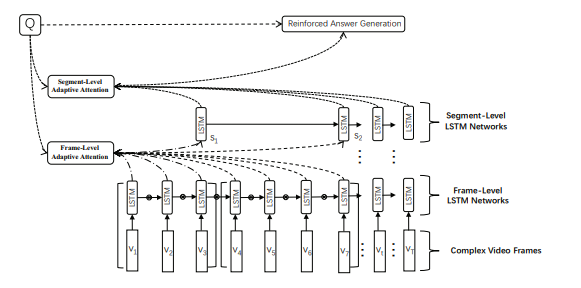
\includegraphics{img/oe.png}
\caption{Open-Ended Long-form Video QA Network}
\end{figure}

The first part is the hierarchical encoder networks that learn the joint
representation of multimodal attentional video and textual question with
adaptive video segmentation.

The second part is the reinforced decoder networks that generate the
natural language answers for open-ended video question answering.

\begin{enumerate}
\def\labelenumi{\arabic{enumi}.}
\setcounter{enumi}{2}
\tightlist
\item
  In this paper, \href{https://arxiv.org/pdf/1805.11752.pdf}{Multi-turn
  Dialogue Response Generation in an Adversarial Learning Framework},
  they propose an adversarial learning approach that can generate
  multi-turn dialogue responses. The network framework that they
  introduce is call \emph{hredGAN} that is based on conditional GANs.
  The generator part of the model is a modified hierachical recurrent
  encoder-decoder network (HRED) and the discriminator is a word-level
  bi-directional LSTM RNN that shares context and word embedding with
  the generator.
\end{enumerate}

During the inference step, noise sampling is conditioned on the dialogue
history and is used to perturb the generator's latent space for
generating possible responses. The final response is the one ranked the
best by the discriminator.

In sum, their hredGAN combines both generative and retrieval-based
multi-turn dialogue systems to improve the model's performance. The
underlying mechanism is that generator and the discriminator share the
context and word embedding and this allows for joint end-to-end training
using back-propogation.

\subparagraph{Summary}\label{summary-2}

Based on our limited research, we found that it is also achievable for
our system to generate the answers for open-ended questions based on the
educational video and provide appropriate feedback/rating for the
learner. The first paper presents a newly developed AES model that can
rate learner's writing. It also demonstrates a possible way of enhance
the AES model by training it with the adversarially crafted input.

In the second paper, we discuss a network that can answer the open-ended
questions based on the video and a given question. Their Adaptive
Hierarchical Reinforced Networks are composed of hierarchical encoder
networks and the reinforced decoder networks. With their framework, we
can easily extend the research topic into educational video specifially.

Similar to the last peper, this paper shows that it is possible to
generate responses conditioned on the context. By leveraging conditional
GAN model framework, their model's performance is significantly
improved.

\subsection{Summary of Learning and Feedback Networks
{[}DRAFT{]}}\label{summary-of-learning-and-feedback-networks-draft}

Based on our previous discussion, we find that both QG and QA (including
VQA) tasks have beem well-researched. A numerous of spcifically designed
algorithms were presented and proved effective for solving these
problems.

There are also some research has been done to tackle both QG and QA
problems at the same time. The research we presented may not be
particularly applicable to the video content. But the implication is
clear, by combining some techniques we learned from the QG and QA
sections separtely with some frameworks like dual learning introduced in
the dual task section, it is plausible for us to conclude that the
coherent QG + QA system for our purpose is not that far-fetched.

As what we anticipated, the research is significantly less in the
open-ended question realm. However, some techniques presented in our
research finding session are very relevant and could certainly serve as
our starting point for solving our problem such as AES model and
open-ended question answering networks. As more and more research comes
out, we should expect more effective solutions to come out soon.

Current reserach is promising but we need more reserach and innovation
in this area.

In open-ended question section, we find that our current research cannot
fully support our goal of taking in the answer in any possible formats
(i.e.~a short video presentation or a recording) besides writing.

\subsubsection{Datasets and Annotation
Needed}\label{datasets-and-annotation-needed}

In order to approach this problem from scratch, we need to create our
own dataset for which we will provide some related resources to start
with:

\begin{enumerate}
\def\labelenumi{\arabic{enumi}.}
\tightlist
\item
  \href{https://research.google.com/youtube8m/}{YouTube-8M Dataset}.
  This is a large-scale labeled video dataset that consists of millions
  of YouTube video IDs, with high-quality generated annotations from a
  diverse vocabulary of 3800+ visual entities. As you can see from its
  introduction, it comes with precomputed audio-visual features from
  billions of frames and audio segments. In short, we can expect the
  following content from this dataset:
\end{enumerate}

\begin{itemize}
\item
  the dataset consists of 6.1M videos URLs, labeled with a vocabulary of
  3863 visual entities
\item
  the video-level dataset comes out to be 18 GB in size, whiel the
  frame-level features are approximately 1.3 TB
\item
  it comes with pre-extracted audio \& visual features from every second
  of video.
\end{itemize}

Though the video content is not limited to education category, we can
still use it to get a strong baseline model.

Naturally, the next step would be constrain our model to train on
particularly educational content. The data needed for taining may
include the raw video clip, annotation/caption of the whole video
content, and audio part of the video.

\begin{enumerate}
\def\labelenumi{\arabic{enumi}.}
\setcounter{enumi}{1}
\tightlist
\item
  In this study
  \href{http://jofdl.nz/index.php/JOFDL/article/download/255/198}{Video
  Captions for Online Courses: Do YouTube's Auto-generated Captions Meet
  Deaf Students' Needs?}, they studied the auto-generated captions
  generated on YouTube online courses. They find that, on average, there
  were 7.7 phrase errors per minute of a total 68 minutes video caption.
  It is been said, we still need to do a lot of annotion work before we
  can finally compose our own training dataset.
\end{enumerate}

Other resources that could possibly help us with out tasks are as below:

\begin{enumerate}
\def\labelenumi{\arabic{enumi}.}
\setcounter{enumi}{2}
\tightlist
\item
  \href{http://videomcc.org/}{VideoMCC}. In their paper, they formulate
  Video Multiple Choice Caption (VideoMCC) as a way to assess video
  comprehension through an easy-to-interpret performance measure. In
  their paper \href{https://arxiv.org/pdf/1606.07373.pdf}{VideoMCC: a
  New Benchmark for Video Comprehension} they propose to cast video
  understanding in the form of multiple choice tests that assess the
  ability of the algorithm to comprehend the semantics of the video.
  Example is as below:
\end{enumerate}

\begin{figure}
\centering
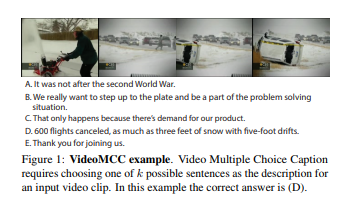
\includegraphics{img/mcc.png}
\caption{VideoMCC}
\end{figure}

\begin{enumerate}
\def\labelenumi{\arabic{enumi}.}
\setcounter{enumi}{3}
\tightlist
\item
  As what we have covered earlier, this paper
  \href{https://arxiv.org/pdf/1512.02902.pdf}{MovieQA: Understanding
  Stories in Movies through Question-Answering}, they introduced a new
  dataset called MovieQA dataset that can evaluate automatic story
  comprehension from both video and text.
\end{enumerate}

Here are 2 figures that can help you better understand their dataset:

\begin{figure}
\centering
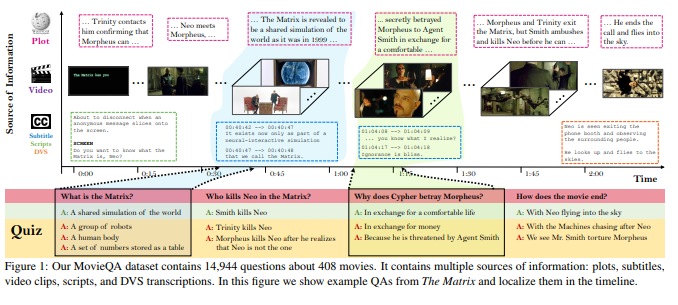
\includegraphics{img/movieqa1.png}
\caption{MovieQA\_1}
\end{figure}

\begin{figure}
\centering
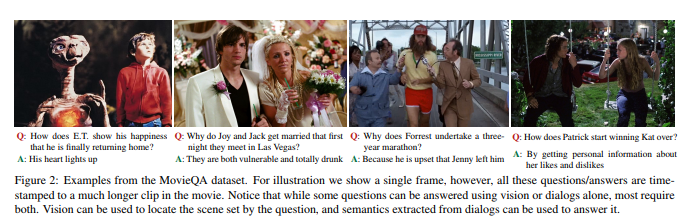
\includegraphics{img/movieqa2.png}
\caption{MovieQA\_2}
\end{figure}

\begin{enumerate}
\def\labelenumi{\arabic{enumi}.}
\setcounter{enumi}{4}
\item
  In this paper \href{https://arxiv.org/pdf/1806.00186.pdf}{Video
  Description: A Survey of Methods, Datasets and Evaluation Metrics}
  mulple methods, datasets and evluation metrics for video description
  task in a comprehensive survey.
\item
  Inspired by this paper
  \href{https://arxiv.org/pdf/1808.07036.pdf}{QuAC : Question Answering
  in Context} in which they present QuAC dataset for QA in Context that
  contains 14K information-seeking QA dialogs such as a student who
  poses a sequence of freeform question to learn as much as possible
  about a hidden Wikipedia text or a teacher who answers the questions
  by providing short excerpts from the text, we are convinced that it is
  might also be possibleob to develop a system that can allow student to
  pause the video and ask our system a information-seeking question and
  then get the answer from our system based on the curent content. .
\end{enumerate}

\section{Knowledge Graph {[}DRAFT{]}}\label{knowledge-graph-draft}

Next, we need to consider how we can select an adequate and relevant
learning masterial and generate an effecive learning map for the
learners based on their current progress and the general knowledge
graph/map, given the ever growing amount of educational content on the
web.

As I mentioned earlier, learning is a knowledge accumulation process.
Knowledge itself has its unique structure that can help us learn in a
most effective and productive way. Knowledge Graph is a great tool that
we developed to map and present the structure of knolwedge. In shirt,
knowledge graphs are collections of relational facts, where each fact
states that a certrain relation holds between 2 entities.

Now we will consider the knowledge graph as the backbone.

\subsection{What is a graph?}\label{what-is-a-graph}

\begin{quote}
Graphs are networks of dots and lines - Graph Theory (Dover Books)
\end{quote}

Mathematically speaking, graphs are mathematical structures used to
model pairwise relations between objects. A graph in this context is
made of vertices, nodes, or points which are connected by edges, arcs or
lines. Typically a graph consists of two sets. A set of vertexes and a
set of edges \[GRAPH_{v,e} =
 \begin{pmatrix}
  v_{1,1} & a_{1,2} & \cdots & a_{1,n} \\
  e_{2,1} & e_{2,2} & \cdots & e_{2,n} \\
 \end{pmatrix}\]

As for the knowledge graph, it is a knowledge base. Often when people
talk about knowledge graph, they are refering to the multi-relational
graph used by Google and its services to enhance search engine's results
with information gathered from a variety of sources. Per Wikipeida,
\href{https://developers.google.com/knowledge-graph/\#knowledge_graph_entities}{Google's
Knowledge Graph} uses a graph database to provide structured and
detailed information about the topic in addition to a list of links to
other sites.

In general, a knowledge graph represents a knowledge domain. It connects
things of different types in a systematic way. Knowledge graphs encode
knowledge arranged in a network of nodes and links rather than tables
and columns. With knolwedge graphs, people and machines can benefit from
a dynamically growing semantic network of facts about things. In other
wrods, we can use it to capture the facts related to people, processes,
applications, data and many other custom ojbects as well as their
relationships among them.

If you want, they can also capture evidence that can be used to
attribute the strengths of these relationships.

Also, we have found a lot of applications that demonstrate that existing
generic knowledge graphs have shown advantages to support semantic
search(i.e.~Google's Knowledge Graph), personal assistant(i.e.~Apple's
Siri) and deep question answering (i.e.~Wolfram Alpha and IBM's Watson).

\subsection{Problem Formulation}\label{problem-formulation-2}

Given we've impletemented the learning and feedback module, knowing
where a given piece of education content fits into the knowledge space
is a vital task if we want the knowledge footprint to make a learner
predictable to others as well as being able to recommend new educational
content that the learner can take on successfully. We will need the
following things to connect educational content.

\begin{quote}
A classifier to take a piece of educational content
\end{quote}

A graph dedicated to education should do the following:

\begin{itemize}
\item
  Provide flexibility for new subjects
\item
  Connect related subjects to each
\item
  Connect concepts related to the content
\item
  Map subject with the Concepts
\end{itemize}

\begin{figure}
\centering
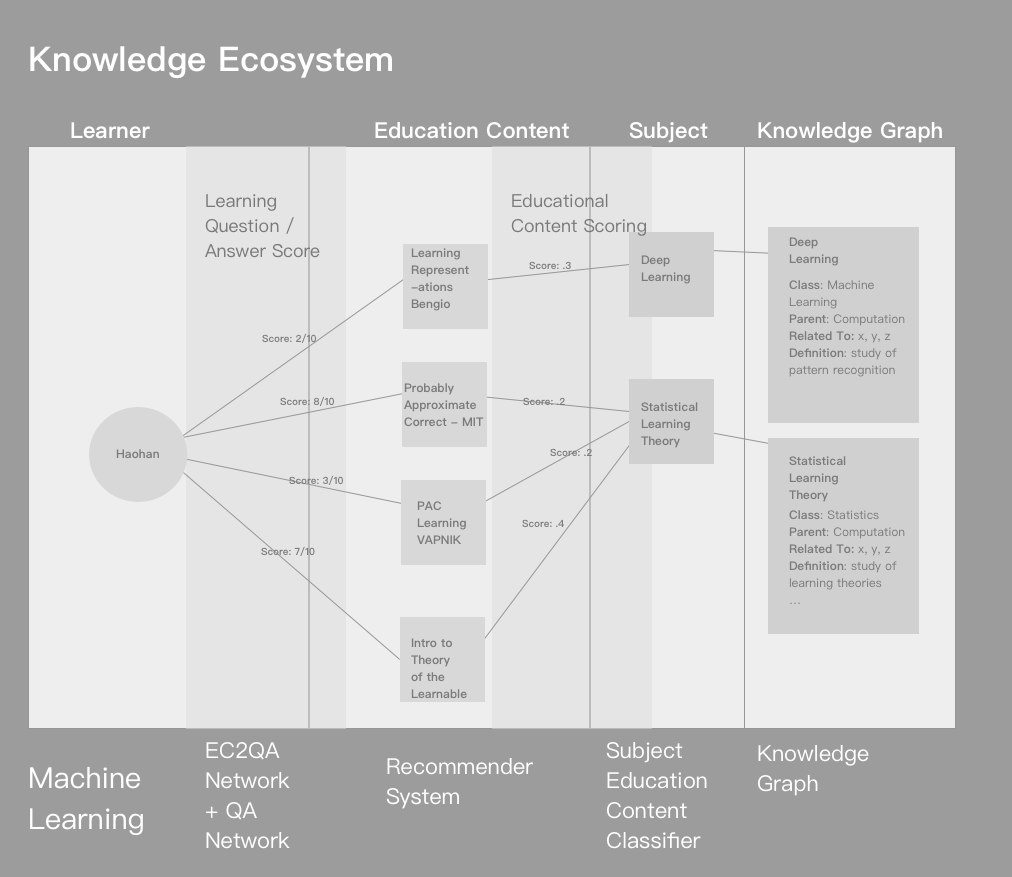
\includegraphics{img/knowledgeEcosystem.png}
\caption{Knowledge Ecosystem}
\end{figure}

\subsection{Key Components}\label{key-components}

Here are some key components that we found important of building an
automated knowledge graph for education:

\begin{enumerate}
\def\labelenumi{\arabic{enumi}.}
\item
  Entity recognition that aims to extract concept of interest from
  structured or unstructured data.
\item
  Relation identification that leverages on the semantic meaning of
  data.
\end{enumerate}

\subsection{Automatic Knowledge Graph
Construction}\label{automatic-knowledge-graph-construction}

Classic knowledge representation techniques allow a knowledge engineer o
create rules that can be interpreted by a reasoner to infer new or
missing triples(subject, predicate, object). These rules are usually
expressed through an ontology which allows for the propagation of
properties from top classes to the lower classes.

However, we are looking for solutions that can allow us to complete our
educational knowledge graph building process. Based on our research,
generic knowledge graphs uaually cannot sufficiently support many
domain-specific applications i.e.~education and finding the
representation of the graph to feed the triples into a machine learning
or deep learning algorithm is still an open area of research. As a
start, let's focus on how to automate the eduction knowledge graph
construction process.

There have been several papers that provide promising results to the
automatation of constructing a knowledge graph. Let's take a look.

\subsection{Case Studies}\label{case-studies-5}

\begin{enumerate}
\def\labelenumi{\arabic{enumi}.}
\tightlist
\item
  In this paper
  \href{https://ieeexplore.ieee.org/document/8362657}{KnowEdu: A System
  to Construct Knowledge Graph for Education}, they propose a system
  KnowEdu that can automatically construct knowledge graph for
  education. In short, the system is able to extract concepts of
  subjects or courses and then identifies the educational relations
  between the concepts.
\end{enumerate}

More importantly, it adopts the neural sequence labeling algorithm on
pedagogical data to extract instruction concepts and employs
probabilistic association rule mining on learning assessment data to
identify the significance of the relations.

In sum, their system consists of the following modules:

\begin{itemize}
\item
  Instructional Concept Extraction Module to extract instructional
  concepts for a given subject or course.
\item
  Educational Relation Identification Module to identify the educational
  relations that interlink instructional concepts to assist the learning
  and teaching process directly.
\end{itemize}

Below is a block diagram of KnowEdu System.

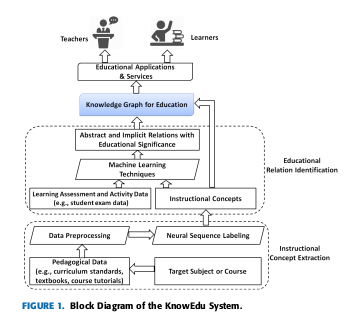
\includegraphics{img/knowedu.png} They used conditional random field
(CRF) model for entity or terminology recognition task. Moreover, they
adopt neural network, or more particularly Gated recurrent unit network
(GRU) architecture for neural sequence labeling on educational entity
extraction task.

In terms of relation identification they implement probabilistic
association data mining techniques on learning assessment adata and
accomplish the task of educational relation identification.

A snapshot of the knowledge graph for mathematics generated by knowedu
system.

\begin{figure}
\centering
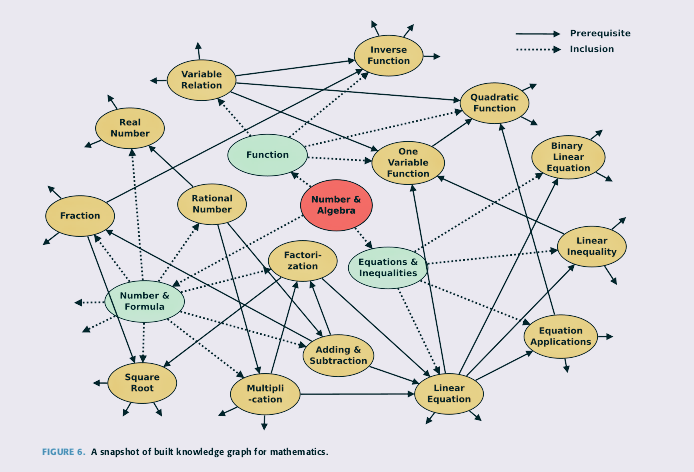
\includegraphics{img/kg.png}
\caption{knowledge\_graph}
\end{figure}

Below are some approaches related to knowledge graph (KG) embedding
which is used to embed components of a KG including entities and
relations into continuous vector space so as to simply the manipulation
while preserving the inherent structure of a KG.

As for its benefits and importance for our task, it can help with a
variety of downstream tasks i.e.~KG completion and relation extraction,
and hence be used to drasically improve the infomration acquisition
speed for KG.

\begin{enumerate}
\def\labelenumi{\arabic{enumi}.}
\setcounter{enumi}{1}
\tightlist
\item
  In this paper
  \href{http://www.mlgworkshop.org/2018/papers/MLG2018_paper_5.pdf}{Generalized
  Embedding Model for Knowledge Graph Mining}, they have presented a
  model for learning neural presentation of generalized knowledge graphs
  using a novel muli-shot unsupervised neural network model, called the
  \textbf{Graph Embedding Network (GEN)}. This model is able to learn
  different types of knowlege graphs from a universal perspective and it
  provides flexibility in learning representations that work on graphs
  conforming to different domains.
\end{enumerate}

In developint their model, they extend the traditional one-shot
supervised learning meachnism by introducing a multi-shot unsupervised
learning framework where a 2-layer MLP network for every shot. This
framework can in turn be used to accommodate both homogeneous and
heterogeneous networks.

\begin{enumerate}
\def\labelenumi{\arabic{enumi}.}
\setcounter{enumi}{2}
\tightlist
\item
  In this paper
  \href{https://openreview.net/pdf?id=rJ4qXnCqFX}{Probabilisic Knowledge
  Graph Embeddings}, they explored a new type of embedding model that
  can link prediction in relational knowledge graph. They start from a
  problem that even large knowledge graphs typically contain only few
  facts per entity, leading effectively to a small data problem where
  parameter uncertainty matters. As for the solution, they suggest that
  the knolwedge graphs should be treated within a Bayesian framework.
\end{enumerate}

In short, they present a probabilistic interpretation of existing
knowledge graph embedding models. By reformulating the models like
ComplEx and DistMult, they construct the generative models for
relational facts.

They also apply stochastic variational inference to scalably estimate an
approximate posterior for each entity and relation embedding in the
knowledge graph. By doing so, they can estimate the uncertainty, but
more importantly, they can use gradient-based hyperparmeter optimization
by stochastic gradient descent on the optimized variational bound.

As a result, their model shows experimentally new state-of-art results
in link prediction task.

\subsection{Summary of Knowledge Graph
{[}DRAFT{]}}\label{summary-of-knowledge-graph-draft}

Based on our research, we are very pleased to see some great progress
has been made to bridge the KG automation process with deep learning and
other machine learning techniques.

As what we discussed above, the first paper introduces a system that
almost exactly matches our goal. The carefully walk us through the
current progress and possible solutions for solving each obstacles in
developing such a educational knowledge graph. For the instructional
concept extraction task, they use both CRF model and neural sequence
labeling algorithm to achieve a high performance. They employ
probabilistic association rule mining on learning assessment data to
identify the relations with educational significance.

The last 2 papers demonstrate the progress that has been made in KG
embedding learning domain. As mentioned above, as one of the most
effective methods in representing knowledge graphs. The development of
this field may offer some great implication for the future KG automation
and acquisition work/research.

\subsubsection{Aatasets and Annotaters
needed}\label{aatasets-and-annotaters-needed}

\begin{enumerate}
\def\labelenumi{\arabic{enumi}.}
\tightlist
\item
  \href{https://ai.google/research/pubs/pub45634}{Knowledge Vault}: A
  web-scale approach to probabilistic knowledge fusion. In this paper
  \href{https://dejanseo.com.au/wp-content/uploads/2014/08/Knowledge-Vault-A-Web-Scale-Approach-to-Probabilistic-Knowledge-Fusion.pdf}{Knowledge
  Vault: A Web-Scale Approach to Probabilistic Knowledge Fusion}, they
  introduce Knowledge Vault that combines extraction from Web content
  (obained through analysis of text, tabular data, page structure, and
  human annotation) with prior knowledge derived from existing knowledge
  repositories.
\end{enumerate}

They employ a supervised machine learning models for fusing these
distinct information sources. As a result, their system can
automatically construct a web-scale probabilistic knowledge base.

\begin{enumerate}
\def\labelenumi{\arabic{enumi}.}
\setcounter{enumi}{1}
\tightlist
\item
  \href{https://developers.google.com/knowledge-graph/\#knowledge_graph_entities}{Google
  Knowledge graph Search API}.
\end{enumerate}

\section{Knowledge Journeys {[}DRAFT{]}}\label{knowledge-journeys-draft}

The knowledge graph is our ground truth and can be applied universally
to some extent, but everyone's learning journey is still highly custom.
In terms of learning, everyone seems to have their unique set of
problems that they are curious about and everyone is on their own
mission towards the mastery. As a result, their knowlege journeys could
have a lot more degree of freedom depends on the learn's learning
history, interests and who they are related to.

We cannot possibly put such an online learning/teaching system into use
without taking this crucial factor into our account. However, this is
not a trivial problem that can be solved with 1 network or 2.

Let's first formulate our problem before we dive into the possible
solutions. Below are few key components that we need to combine to
achieve our ultimate goal which is to appropriately guide the learner
through their unique knowledge journey:

\begin{enumerate}
\def\labelenumi{\arabic{enumi}.}
\tightlist
\item
  First, we need to
\end{enumerate}

, we can rely on some heuristic and models that have been developed to
resolve this type of idiosymcratic issue.

As we all know that a recommender system is an intuitive line of defense
against consumer over-choice given the evern growing information
available on the web. As we mentioned earlier in the knowledge graph, a
authoritative and personalized recommending system is essential for
facilitating the learning.

Typically, a recommendation models can be classified into 3 main
categories:

\begin{enumerate}
\def\labelenumi{\arabic{enumi}.}
\item
  Collaborative filtering
\item
  Content based
\item
  Hybrid recommender system
\end{enumerate}

As I mentioned, here we will mainly focus on hybrid recommender system.

There are a diverse array of achitectual paradigms that are closely
related recommending system. Let's take a look at few of them: 1.
Autoencoder

\begin{enumerate}
\def\labelenumi{\arabic{enumi}.}
\setcounter{enumi}{1}
\item
  Convolutional Neural Network
\item
  Recurrent Neural Network
\item
  Restricted Boltzmann Machine (RBM)
\item
  Adversarial Networks
\item
  Attentional Models (AM)
\item
  Deep Reinforcement Learning (DRL)
\end{enumerate}

\subsection{Summary of Current Research and Needs
{[}DRAFT{]}}\label{summary-of-current-research-and-needs-draft}

\section{Data and Annotation
{[}DRAFT{]}}\label{data-and-annotation-draft}

\subsection{Reference {[}DRAFT{]}}\label{reference-draft}

\begin{enumerate}
\def\labelenumi{\arabic{enumi}.}
\item
  \href{https://arxiv.org/pdf/1808.04961.pdf}{A Framework for Automatic
  Question Generation from Text using Deep Reinforcement Learning}
\item
  \href{https://arxiv.org/pdf/1705.00106.pdf}{Learning to Ask: Neural
  Question Generation for Reading Comprehension}
\item
  \href{http://openaccess.thecvf.com/content_ECCV_2018/papers/Yalong_Bai_Deep_Attention_Neural_ECCV_2018_paper.pdf}{Deep
  Attention Neural Tensor Network for Visual Question Answering}
\item
  \href{http://www.cs.cornell.edu/~xdu/papers/acl17_dsc_poster.pdf}{Learning
  to Ask}
\item
  \href{https://openreview.net/pdf?id=rk3pnae0b}{TOPIC-BASED QUESTION
  GENERATION}
\item
  \href{https://arxiv.org/pdf/1707.07435.pdf}{Deep Learning based
  Recommender System}
\end{enumerate}

\chapter{Challenges}\label{challenges}

We have listed one approach to better represent a modern individual's
knowledge by taking the world of unstructured educational content and
generating a way to test a learner's knowledge and a way to to map the
content to an education based knowledge graph. We surveyed the relevant
machine and deep learning research, introduced EC2QA, a novel network
for taking in educational content and generate questions, answers, as a
knowledge evaluation mechanism, and introduced the knowledge system
consisting of the knowledge footprint, knowledge graph, and knowledge
journeys to help support a learner's knowledge acquistion,
representation, and a way to look at an improved way to view society's
collective knowledge.

\begin{itemize}
\tightlist
\item
  Datasets -- EC2QA dataset -- Knowledge graph dataset
\item
  Deep Learning Architecture -- EC2QA network
\end{itemize}

\section{Creating a research dataset}\label{creating-a-research-dataset}

\section{Collaboration with education
technologists}\label{collaboration-with-education-technologists}

\chapter{Conclusion}\label{conclusion}

In conclusion, we presented a new perspective on knowledge acquistion,
representation, and proposed an ecosystem that would support a modern
and adaptative knowledge ecosystem.

Our main task was to take an individual and begin to get a true
depiction of their knowledge beyond their traditional degree which is
only a small percentage of someone's education. We focused on taking the
world of unstructured educational content online, and how to provide
structure in the form of testing and mapping it to a knowledge graph.

There is still much research to be done in bringing to life the EC2QA
network as well as the data needed and the collaboration needed amongst
machine learning researchers, teachers, and designers needed.

As machine learning researchers we are looking forward to building our
next prototype and collaborating around this work.

\chapter{About Authors}\label{about-authors}

\section{Haohan Wang}\label{haohan-wang}

\section{Fanli Zheng (Christian
Ramsey)}\label{fanli-zheng-christian-ramsey}

\section{Contact}\label{contact}

Feel Free to contact us if you have any question: Visit our website
dyadxmachina.com

Haohan Wang:
\href{mailto:haohan723@gmail.com}{\nolinkurl{haohan723@gmail.com}}

Christian Fanli Ramsey:
\href{mailto:thechristianramsey@gmail.com}{\nolinkurl{thechristianramsey@gmail.com}}

\chapter{References}\label{references}

\chapter{CR Knowledge Graph}\label{cr-knowledge-graph}

Now we will consider the knowledge graph as the backbone.

\section{What is a graph?}\label{what-is-a-graph-1}

\begin{quote}
Graphs are networks of dots and lines - Graph Theory (Dover Books)
\end{quote}

Mathematically speaking a graph consists of two sets. A set of vertexes
and a set of edges \[GRAPH_{v,e} =
 \begin{pmatrix}
  v_{1,1} & a_{1,2} & \cdots & a_{1,n} \\
  e_{2,1} & e_{2,2} & \cdots & e_{2,n} \\
 \end{pmatrix}\]

Google's Knowledge Graph Google Knowledge Vault

Problem Formulation

Given we've impletemented the learning and feedback module, knowing
where a given piece of education content fits into the knowledge space
is a vital task if we want the knowledge footprint to make a learner
predictable to others as well as being able to recommend new educational
content that the learner can take on successfully. We will need the
following things to connect educational content.

\begin{quote}
A classifier to take a piece of educational content
\end{quote}

What we need

A graph dedicated to education should do the following: - Provide
flexibility for new subjects - Connect related subjects to each -
Connect concepts

Subject -\textgreater{} Concepts

\section{Automatic Knowledge Graph
Construction}\label{automatic-knowledge-graph-construction-1}

There have been several papers that provide promising results to the
automatation of constructing a knowledge graph but not as many in the
domain of education.

\section{Concept Extraction}\label{concept-extraction}

\section{Relation Extraction}\label{relation-extraction}

\subsection{Summary of Current Research and Needs
{[}DRAFT{]}}\label{summary-of-current-research-and-needs-draft-1}

\section{Data and Annotation
{[}DRAFT{]}}\label{data-and-annotation-draft-1}

\subsection{Reference {[}DRAFT{]}}\label{reference-draft-1}

\begin{enumerate}
\def\labelenumi{\arabic{enumi}.}
\item
  \href{https://arxiv.org/pdf/1808.04961.pdf}{A Framework for Automatic
  Question Generation from Text using Deep Reinforcement Learning}
\item
  \href{https://arxiv.org/pdf/1705.00106.pdf}{Learning to Ask: Neural
  Question Generation for Reading Comprehension}
\item
  \href{http://openaccess.thecvf.com/content_ECCV_2018/papers/Yalong_Bai_Deep_Attention_Neural_ECCV_2018_paper.pdf}{Deep
  Attention Neural Tensor Network for Visual Question Answering}
\item
  \href{http://www.cs.cornell.edu/~xdu/papers/acl17_dsc_poster.pdf}{Learning
  to Ask}
\item
  \href{https://openreview.net/pdf?id=rk3pnae0b}{TOPIC-BASED QUESTION
  GENERATION}
\item
  \href{https://arxiv.org/pdf/1707.07435.pdf}{Deep Learning based
  Recommender System}
\end{enumerate}

\bibliography{book.bib,packages.bib}


\end{document}
